\documentclass[twoside]{article}

%\usepackage{aistats2021}
% If your paper is accepted, change the options for the package
% aistats2021 as follows:
%
\usepackage[accepted]{aistats2021}
\usepackage{amsfonts}
\usepackage{graphicx}
\usepackage{multirow}
%
% This option will print headings for the title of your paper and
% headings for the authors names, plus a copyright note at the end of
% the first column of the first page.

% If you set papersize explicitly, activate the following three lines:
%\special{papersize = 8.5in, 11in}
%\setlength{\pdfpageheight}{11in}
%\setlength{\pdfpagewidth}{8.5in}

% If you use natbib package, activate the following three lines:
\usepackage{natbib}
%\renewcommand{\bibname}{References}
%\renewcommand{\bibsection}{\subsubsection*{\bibname}}

% If you use BibTeX in apalike style, activate the following line:
%\bibliographystyle{apalike}

\begin{document}

% If your paper is accepted and the title of your paper is very long,
% the style will print as headings an error message. Use the following
% command to supply a shorter title of your paper so that it can be
% used as headings.
%
%\runningtitle{I use this title instead because the last one was very long}

% If your paper is accepted and the number of authors is large, the
% style will print as headings an error message. Use the following
% command to supply a shorter version of the authors names so that
% they can be used as headings (for example, use only the surnames)
%
%\runningauthor{Surname 1, Surname 2, Surname 3, ...., Surname n}

\twocolumn[

\aistatstitle{TDHNN: Time-Dependent Hamiltonian Neural Networks }

\aistatsauthor{ Shaan A. Desai$^{1,2}$ \And David Sondak$^{2}$ \And  Marios Mattheakis$^{2}$ }

\aistatsaddress{ Machine Learning Research Group \\University of Oxford $^1$ \And Institute of Applied Computational Science \\ Harvard University $^2$ } ]


\bibliographystyle{abbrv}
\begin{abstract}

Deep neural-networks embedded with physically-informed priors demonstrate remarkable performance over vanilla neural-networks in accurately learning and predicting non-linear dynamical systems. Recently, it was shown that Hamiltonian Neural Networks (HNNs) - neural networks designed to conserve energy and exploit the Hamiltonian formalism, show strong and consistent performance in learning autonomous systems that depend implicitly on time. Here, we extend this framework to include an explicit time-dependence that generalizes the learning to non-autonomous dynamical systems. We achieve this generalisation by embedding a modified Port-Hamiltonian into our neural networks that extends the general Hamiltonian to capture damped and forced systems alike. We show that our network can learn systems as complex as the duffing equation in the chaotic regime while maintaining comparable performace to HNNs in settings with no explicit time-dependence.

%Unlike vanilla Artificial Neural Networks, Neural Networks embedded with physically-informed priors achieve remarkable results in accurately learning and predicting non-linear dynamical systems.
% despite this success, their generalization is often limited by the available training data which in practice only consists of a few short-range trajectories. naturally we might ask how we can generalize to unseen timesteps better?
% Despite this success, their generalization performance is often limited to short-range trajectories that run for less than the final training time. The performance degradation is due to state and energy drift induced by errors accumulating over time and it poses a critical challenge to learning highly non-linear and chaotic long-range dynamics precisely when data for only a limited number of short-range trajectories are available. One proposed solution to this challenge has been to incorporate symplectic integrators that aim to preserve the symplectic flow. Here, we present an alternative, an L1 penalty of the Hamiltonian derivative with respect to time: $d\mathcal{H}(p,q,t)/dt$. The inclusion of this term, a straightforward addition to the network, enforces the Hamiltonian to remain constant in time for a given trajectory. We empirically illustrate the stabilising effect this penalty has on our network. In addition, we use it solve problems in non-linear dynamics such as heinon-heiles, 3-body problem and double pendulum.
\end{abstract}

\begin{figure*}[ht!]
\centering
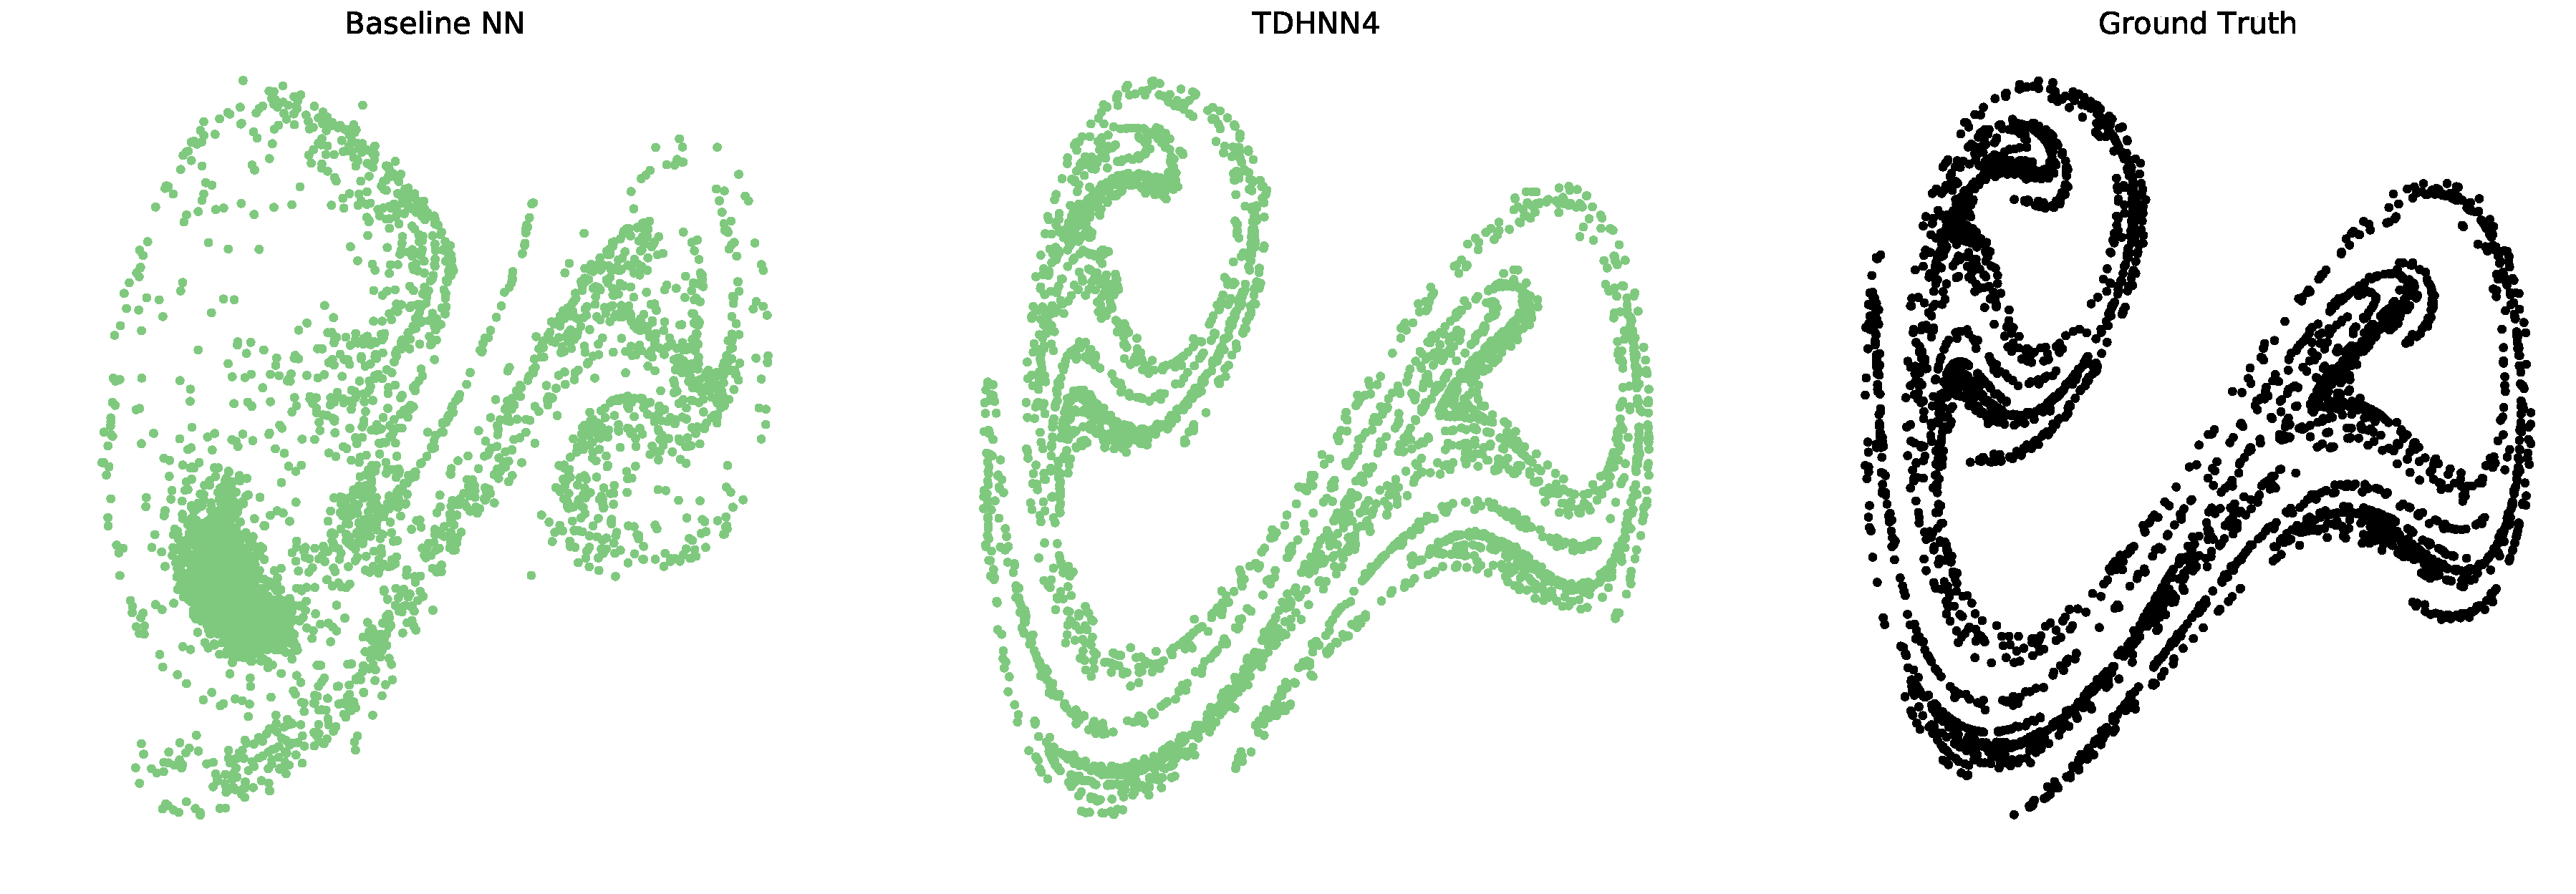
\includegraphics[width=0.9\textwidth]{figures/main_fig.pdf}
\caption{Poincar\'e Sections of a duffing oscillator in a chaotic regime. Both Baseline NN and TDHNN4 are trained for 20000 iterations with 2000 data points. TDHNN4 significantly outperforms Baseline NN at recovering the ground truth Poincar\'e section.}
\end{figure*}
\label{fig.chaos}
\section{Introduction}

Neural networks (NNs), as universal function approximators \cite{hornik_multilayer_1989}, have shown resounding success across a host of domains. However, their performance in learning physical systems has often been limited. New research in \textit{scientific machine learning} - a branch that tackles scientific problems with domain-specific machine learning methods, is paving a way to address these challenges. For example, it has been shown that prior theoretical information embedded in networks, such as Hamiltonian mechanics \cite{greydanus_hamiltonian_2019}, Lagrangians \cite{cranmer_lagrangian_2020, lutter_deep_2019}, Ordinary Differential Equations (ODEs) \cite{chen_neural_2018}, physics equations \cite{raissi_physics_2017} and Graph Neural Networks \cite{battaglia_interaction_2016,sanchez-gonzalez_hamiltonian_2019} can significantly improve learning in complex physical domains. Furthermore, it has been shown that such systems can be adapted to learn trajectories of controlled dynamics \cite{lutter_deep_2019,zhong_dissipative_2020}. Despite this extensive research, there is still no method that accounts for explicit-time dependence, a crucial component in forced dynamical systems. Additionally, many of the existing approaches present no direct way to account for dissipation. Inspired by \cite{zhong_dissipative_2020}, we show that a Port-Hamiltonian - a method designed to account for forcing and dissipation, can be used to learn the dynamics of explicit time-dependent physical systems. We benchmark our network on a range of tasks from the simple mass-spring system to a chaotic duffing equation. Our network consistently outperforms other approaches while actively learning both the driving force and damping coefficient. We also show that our network can visually recover the Poincar\'e section of a duffing equation in the chaotic regime Fig.\ref{fig.chaos}.

\section{Background}

\subsection{Hamiltonian Neural Networks}

Recently, \cite{greydanus_hamiltonian_2019} demonstrated that dynamic predictions through time can be improved using Hamiltonian Neural Networks (HNNs) which endow models with a Hamiltonian constraint. The Hamiltonian is an important representation of a dynamical system because it is one of two well-known approaches that generalizes classical mechanics. The Hamiltonian $\mathcal{H}$ is a scalar function of position $\mathbf{q} = (q_1,q_2,....,q_M)$ and momentum $\mathbf{p} = (p_1,p_2,....,p_M)$. It is a powerful representation because it allows us to obtain the time derivatives of the inputs $(\dot{\mathbf{q}},\dot{\mathbf{p}})$ by simply differentiating the Hamiltonian with respect to its inputs (see Eqn.\ref{eqn.hamiltonian}.)
\begin{equation}
\frac{\mathrm{d}\mathbf{q}}{\mathrm{d}t} = \frac{\partial \mathcal{H}}{\partial \mathbf{p}}, ~~~
\frac{\mathrm{d}\mathbf{p}}{\mathrm{d}t} = -\frac{\partial \mathcal{H}}{\partial \mathbf{q}}
\label{eqn.hamiltonian}
\end{equation}
As a consequence, it is noted in \cite{greydanus_hamiltonian_2019} that by parametrizing the Hamiltonian with a neural network e.g. $H_{\theta}(\mathbf{q},\mathbf{p})$ where $\theta$ represents a deep neural network, one can easily obtain the system's dynamics by differentiating (via autograd) the Hamiltonian with its inputs. This information allows us to build two 1st-order differential equations which can be used to update the state space, $(\mathbf{q},\mathbf{p})$. Equation \ref{eqn.action_int} shows this integral, in which we define the symplectic gradient $\mathbf{S}  = \left [ \frac{\partial \mathcal{H}}{\partial \mathbf{p}},-\frac{\partial \mathcal{H}}{\partial \mathbf{q}} \right ] $:
\begin{equation}
(\mathbf{q},\mathbf{p})_{t+1} = (\mathbf{q},\mathbf{p})_t + \int_t^{t+1} \mathbf{S}(\mathbf{q},\mathbf{p}) \mathrm{d}t
\label{eqn.action_int}
\end{equation}
However, this is not the only benefit in learning a Hamiltonian. Another key attribute of the Hamiltonian is that the vector field $\mathbf{S}$ is a symplectic gradient meaning $\mathcal{H}$ remains constant as long as state vectors are integrated along $\mathbf{S}$. This result links the Hamiltonian with the total energy of the system such that $\mathcal{H}(\mathbf{q},\mathbf{p}) = E_{tot}$ for many physical systems. Therefore, the Hamiltonian is a powerful inductive bias that can be utilised to evolve a physical state while maintaining energy conservation. 

Although this formalism is compact and powerful, it does not readily generalize to damped or forced system. As such, we refer to port-Hamiltonian systems.

\subsection{Port-Hamiltonians}

Port-Hamiltonians are a formalism that allow us to correct Hamilton's equations to incorporate damping and forcing terms. The first method to embed the port-Hamiltonian in a neural network \cite{zhong_dissipative_2020} shows how to represent a general form for such a system. In \cite{zhong_dissipative_2020} the Port-Hamiltonian is represented as:
\begin{equation}
\resizebox{0.9\linewidth}{!}{$%
\begin{bmatrix}
\dot{\mathbf{q}} \\
\dot{\mathbf{p}}
\end{bmatrix}
=
\Bigg(\begin{bmatrix}
0 & \mathbf{I} \\
-\mathbf{I} & 0
\end{bmatrix} +
\mathbf{D}_{\theta_2}(\mathbf{q})
 \Bigg)
 \begin{bmatrix}
\frac{\partial \mathcal{H}_{\theta_1}}{\partial \mathbf{q}} \\
\frac{\partial \mathcal{H}_{\theta_1}}{\partial \mathbf{p}}
\end{bmatrix}
+
\begin{bmatrix}
0 \\
\mathbf{g}(\mathbf{q})
\end{bmatrix}
u
$%
}%
\label{eqn.pham}
\end{equation}
where $\mathbf{D}_{\theta_2}(\mathbf{q})$ is the damping term and $g(q)u$ is the external constant control term. 

This general formalism allows us to collapse to classical Hamiltonians by simply setting $\mathbf{D}$ and $u$ to zero. Note here that the authors of \cite{zhong_dissipative_2020} assume the vector $[\mathbf{q},\mathbf{p},u]$ is provided as input to the system. The matrix $\mathbf{D}_{\theta_2}(\mathbf{q})$ is assumed to be semi-positive definite and $g(q)$ is typically a non-linear scaling of $q$ to account for polynomial scaling of forces, for example, as would be found in the Hill-Schroedinger equation.

\section{Related Work}

Numerous recent methods show how to learn dynamics via physically informed priors.
\subsection{Functional Priors}
Functional priors typically embed the full functional form of an equation, into the neural network. Physics-informed Neural Networks (PINNs) \cite{raissi_physics_2017,raissi_physics-informed_2019} and Hamiltonian Nets (Marios) look at directly embedding the equations into the loss function. PINNs furthermore exploit autograd to compute partial-derivatives and show that such an approach is more powerful than symbolic regression.

\subsection{Integrator Priors}
Many methods seek to use a NN to parametrize the derivatives $\dot{S}$ of a state $S$ and then use this learned parametrization in a scientific integrator such as a Runge-Kutta method. The authors of NeuralODE \cite{chen_neural_2018} show that the embedding of the integrator in the learning process induces a continuous depth neural network for large time-step predictions. As such, the number of gradient computations scales exponentially. The paper re-introduces the adjoint method to ensure linear scaling of the gradient computations. Other work such as \cite{zhu_deep_2020} theoretically proves that the embedded integrator in Hamiltonian Neural Networks significantly benefits from being symplectic. 

\subsection{Graph based methods}
In \cite{battaglia_interaction_2016}, the authors show how a Graph Neural Network, designed to capture the relational structure of systems, can be used to learn interacting particle systems. This work has been exploited in numerous advances \cite{sanchez-gonzalez_graph_2018,sanchez-gonzalez_learning_2020,cranmer_lagrangian_2020}.

\subsection{Lagrangian/Hamiltonian Methods}
While \cite{cranmer_lagrangian_2020} and \cite{greydanus_hamiltonian_2019} propose the explicit learning of Hamiltonian and Lagrangian functions, \cite{lutter_deep_2019} shows how one can exploit the Lagrangian equation to learn both a function which can predict the generalized forces as well as use generalized forces and coordinate information to predict the next state. The authors show that their inverse model can accurately predict a controlled double pendulum, which is pertinent for controlled robots.


\subsection{Latest Advances}
CHNN \cite{finzi_generalizing_2020}, one of the most recent advances published as a spotlight in NeurIPS 2020, looks at enforcing cartesian coordinates in Hamiltonians and Lagrangians with holonomic constraints. The paper emphasises that such a framework works significantly better at learning deeply complex physical systems such as the 5-pendulum. 

Our method investigates a more general Hamiltonian formalism, and similar to \cite{finzi_generalizing_2020}, explicitly encodes the holonomic constraints into the network.

\section{Method}

The architecture for our method can be seen in Fig.\ref{fig.architecture}. We modify the Port-Hamiltonian in Eqn.\ref{eqn.pham} in two ways. First, we know that many physical systems have a damping matrix that only consists of a non-zero, state-independent term in the lower right quadrant, so we replace $\mathbf{D}(\mathbf{q})$ with a single weight parameter independent of $\mathbf{q}$ in the lower right half of the matrix. Secondly, we set $g(q)=1$ and replace $u$ with $F_{\theta_3}(t)$ as many physical systems of interest do not typically scale the force by non-linear $q$ terms as can be found in the examples in \cite{zhong_dissipative_2020}. The resulting equation is:

\begin{equation}
\resizebox{0.9\linewidth}{!}{$%
\begin{bmatrix}
\dot{\mathbf{q}} \\
\dot{\mathbf{p}}
\end{bmatrix}
=
\Bigg(\begin{bmatrix}
0 & \mathbf{I} \\
-\mathbf{I} & 0
\end{bmatrix} +
\begin{bmatrix}
0 & 0 \\
0 & \mathbf{D}_{\theta_2}
\end{bmatrix}
 \Bigg)
 \begin{bmatrix}
\frac{\partial \mathcal{H}_{\theta_1}}{\partial \mathbf{q}} \\
\frac{\partial \mathcal{H}_{\theta_1}}{\partial \mathbf{p}}
\end{bmatrix}
+
\begin{bmatrix}
0 \\
\mathbf{F}_{\theta_3}(\mathbf{t}))
\end{bmatrix}
$%
}%
\label{eqn.pham1}
\end{equation}

Although we have made some simplifying assumptions, our method remains versatile at capturing the underlying form of many complex physical phenomena. 

\begin{figure}[h!]
\centering
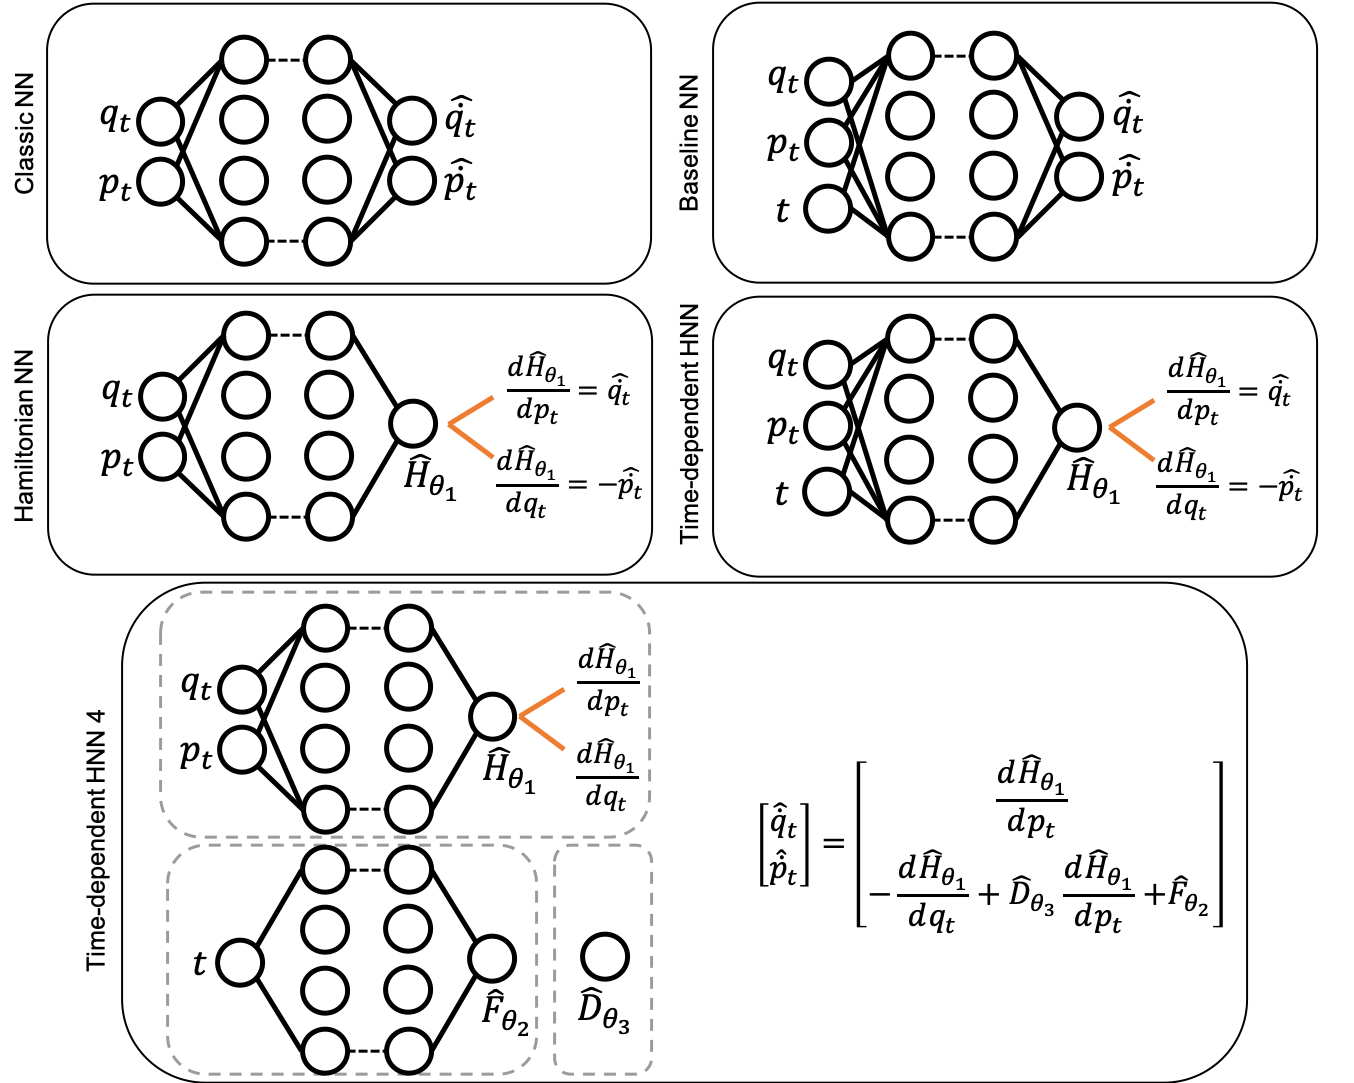
\includegraphics[width=0.5\textwidth]{figures/architect.png}
\caption{Architectures used to learn dynamics in this paper. The naive extension of classic NN and Hamiltonian NN (top left) is to incorporate time as an additional input variable (top right). Our innovation, which exploits Port-Hamiltonians, explicitly learns the force $F_{\theta_2}$ as well as the damping coefficient $D_{\theta_3}$.}
\label{fig.architecture}
\end{figure}

We define the loss function for our architecture as follows:
\begin{equation}
\resizebox{0.9\linewidth}{!}{$%
\mathcal{L} =\left\| \frac{\partial \mathcal{H}_{\theta_1}}{\partial \mathbf{q}} +  \frac{\partial \mathbf{p}}{\partial t} \right\| +\left\| \frac{\partial \mathcal{H}_{\theta_1}}{\partial \mathbf{p}} -  \frac{\partial \mathbf{q}}{\partial t} \right\|+ \alpha_{reg}| \mathbf{F}_{\theta_3} (\mathbf{t})| + \beta_{reg}|\mathbf{D}_{\theta_2}| 
$%
}
\end{equation}

To learn the dynamics, we feed in a state-vector $\mathbf{S}_t = [\mathbf{q},\mathbf{p},\mathbf{t}]$ to our model. The first neural-network $\mathcal{H}_{\theta_1}$ consists of 3 hidden layers designed to predict $\mathcal{H}$ from $[\mathbf{q},\mathbf{p}]$ data. The second component $\mathbf{D}_{\theta_2}$ consists of a single weight parameter designed to learn the damping coefficient $\mathbf{D}$ and the third neural-network consists of 2 hidden layers designed to predict $\mathbf{F(\mathbf{t})}$. We use an L2-norm penalty for the predicted state-vectors and an L1-norm for force and damping to encourage sparsity. We do this because we would like our networks to identify classical autonomous systems (which may not have force or time) as well as non-autonomous systems. For our experiments we use 200 hidden layers and find that most activations, including tanh, sin and cos yield comparable results. To benchmark our method, as \cite{greydanus_hamiltonian_2019} do, we use a modified classic NN that takes in an additional time vector and predicts $[\dot{q},\dot{p}]$. We also take the straightforward extension of HNN to include time as a variable input. At inference, we use a Runge-Kutta 4th order integrator to rollout the initial conditions. 

\section{Results}

We benchmark the performance of our models on numerous datasets that canvas time-independent systems to complex chaotic forced systems.

\subsection{Simple Mass Spring}

The simple mass spring system is a well known system from classical physics that obeys Hooke's Law. The Hamiltonian for a simple mass spring system is written as:

\begin{equation}
\mathcal{H} = \frac{1}{2}k\mathbf{q}^2 + \frac{1}{2m}\mathbf{p}^2 
\end{equation}

For simplicity, we set $k$ and $m$ to 1 for our experiments. We sample 25 initial training conditions such that r in $q^2+p^2 = r^2$ is between 0.5 and 1.5 as is done in \cite{greydanus_hamiltonian_2019}. The trajectories are sampled with $\delta t =0.05$ and $T_{max} = 3.05$.  The test error in fig.\ref{mspring} is measured as a Mean Squared Error (MSE) be across for 50 trajectories. We investigate this simple system to show that learning a separate, regularised forcing term results in much better state and energy rollout in comparison to TDHNN and baseline NN. The main reason for this is that while TDHNN and baseline NN will learn dynamics with time-steps within the training regime, they typically cannot generalize to unseen timesteps. Learning a separate forcing term and regularizing it keeps the time component independent of the Hamiltonian and therefore allows us to nearly match the performance of HNN.

\begin{figure}[h!]
\centering
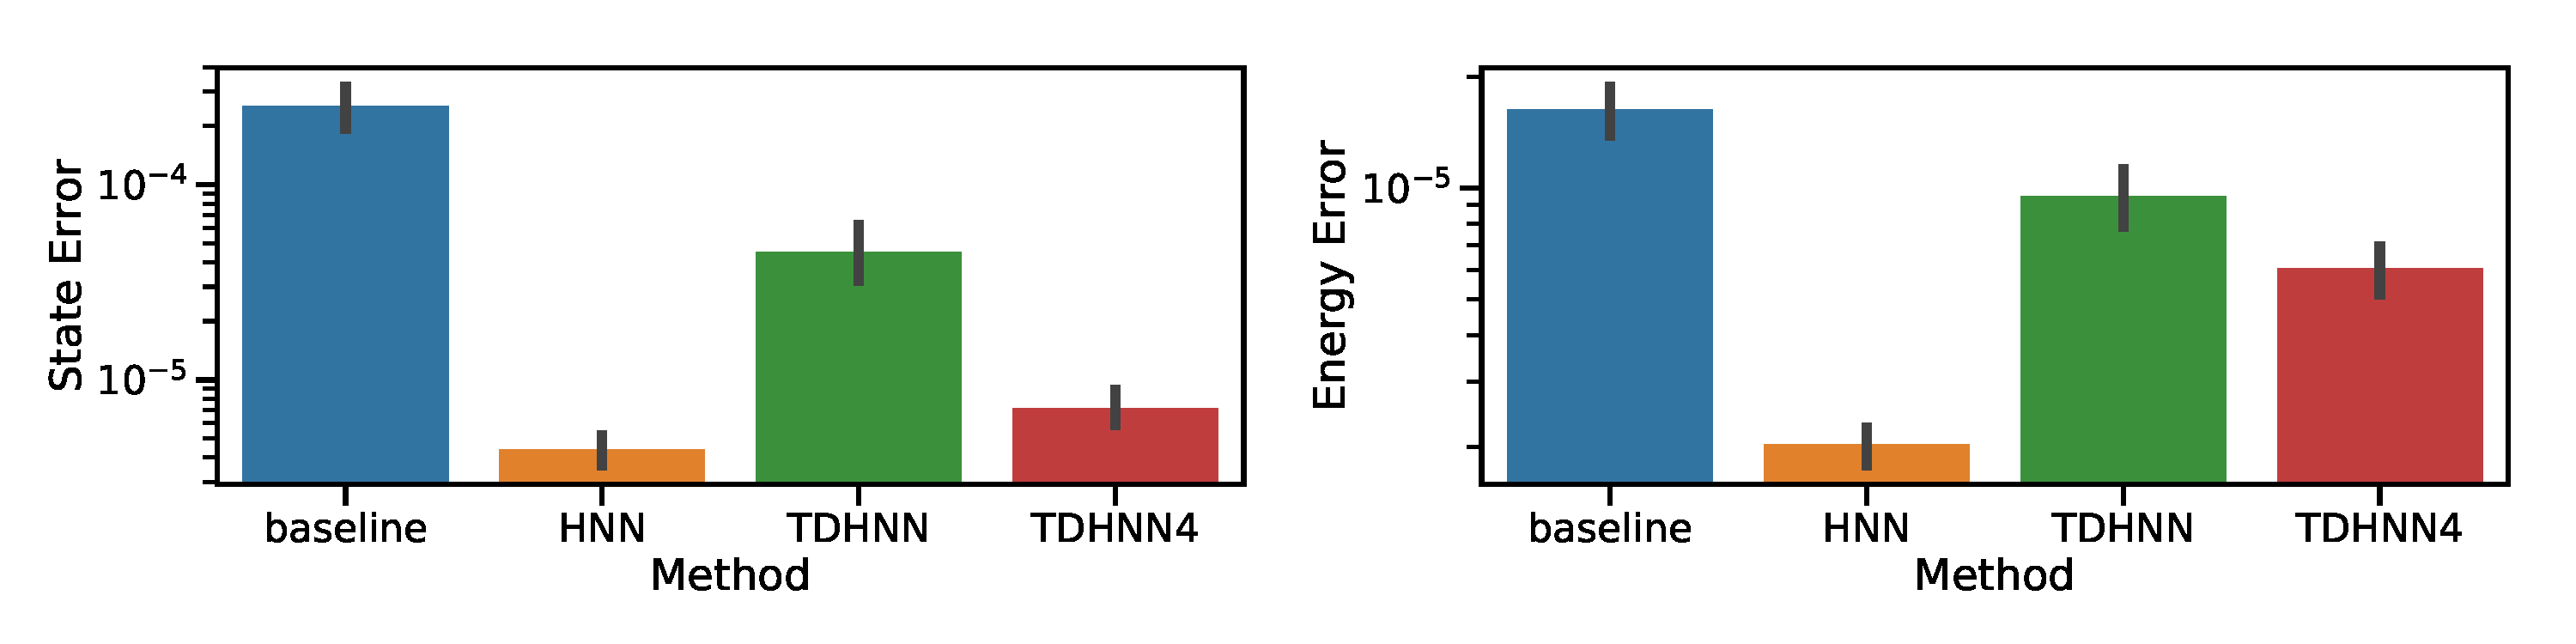
\includegraphics[width=0.5\textwidth]{figures/mass_spring_errors.pdf}
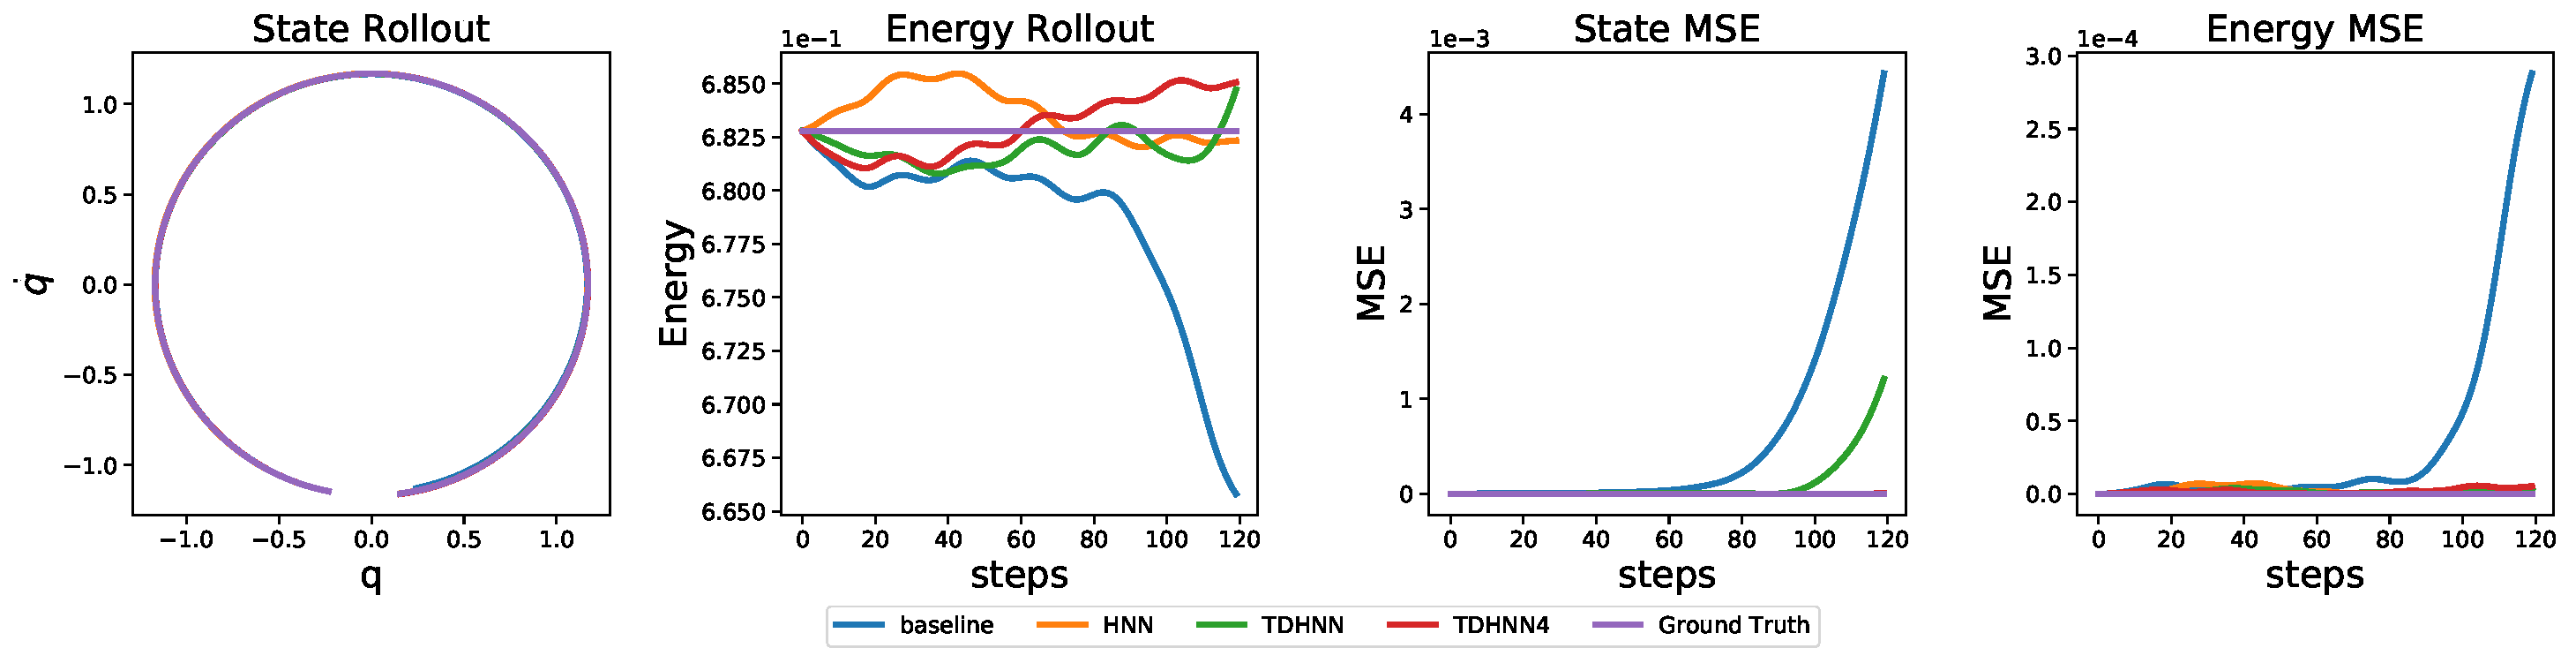
\includegraphics[width=0.5\textwidth]{figures/mass_spring_long.pdf}
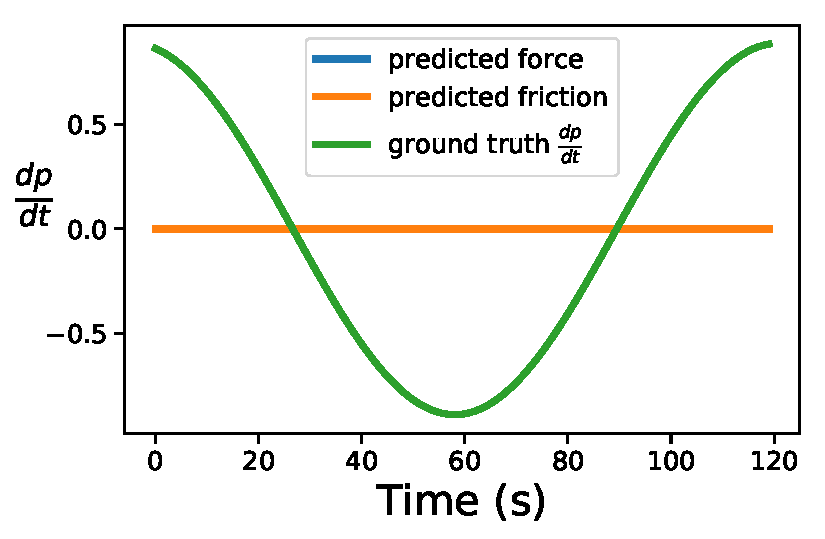
\includegraphics[width=0.4\textwidth]{figures/mass_spring_pred_force.pdf}
\caption{Simple Mass Spring system has no explicit time dependence. We see that TDHNN4 can almost recover the dynamics of HNN which doesn't depend on time. The result is achieved by regularising the force and friction terms as can be seen in the bottom figure. Baseline and TDHNN are unable to achieve the same state-error as their time-dependence }
\label{mspring}
\end{figure}


\subsection{Damped Mass Spring}

Damping is generally not considered part of Hamiltonian systems. For example, let us take the following damped system:
\begin{equation}
\ddot{\mathbf{q}} = -\mathbf{q} - \delta\dot{\mathbf{q}}
\end{equation}
and we know $\mathbf{p}=m\dot{\mathbf{q}}$ which implies $\dot{\mathbf{q}} = m^{-1}\mathbf{p}$.

Then, the integral of the right hand side with respect to q will give us:

\begin{equation}
\frac{\mathbf{q}^2}{2} + \delta \mathbf{q} \dot{\mathbf{q}}
\end{equation}

The equation above looks like a modified potential function which can be combined with a kinetic energy term to give a Hamiltonian as:

\begin{equation}
\mathcal{H} =\frac{ \mathbf{p}^2}{2m} + \frac{\mathbf{q}^2}{2} + \delta \mathbf{q} \dot{\mathbf{q}}
\end{equation}

However, although we can recover the differential equation for $\ddot{\mathbf{q}}$ by $-\frac{\partial\mathcal{H}}{\mathrm{d}\mathbf{q}}  =-\mathbf{q} - \delta\dot{\mathbf{q}} = \ddot{\mathbf{q}}$, we violate the rule that $\dot{\mathbf{q}} = m^{-1}\mathbf{p}$ since $ \frac{\partial\mathcal{H}}{\mathrm{d}\mathbf{p}} =  \dot{\mathbf{q}} +\delta \mathbf{q} \neq \dot{\mathbf{q}} $.


However, as we saw with Port-Hamiltonians, there is a straightforward way to account for the damping term without explicitly defining a full Hamiltonian. By combining a regular Hamiltonian with an additional term that learns the damping, we can disentangle the two terms for learning.

For training, we have 20 initial conditions, uniformly sampled in $[-1,1]^2$. Each trajectory is evolved until $T_{max} = 30.1$ with a $\delta t = 0.1$. At inference, we compute the rollout of 25 trajectories, and report the average state and energy rollout MSE in fig.\ref{damped}.

\begin{figure}[h!]
\centering
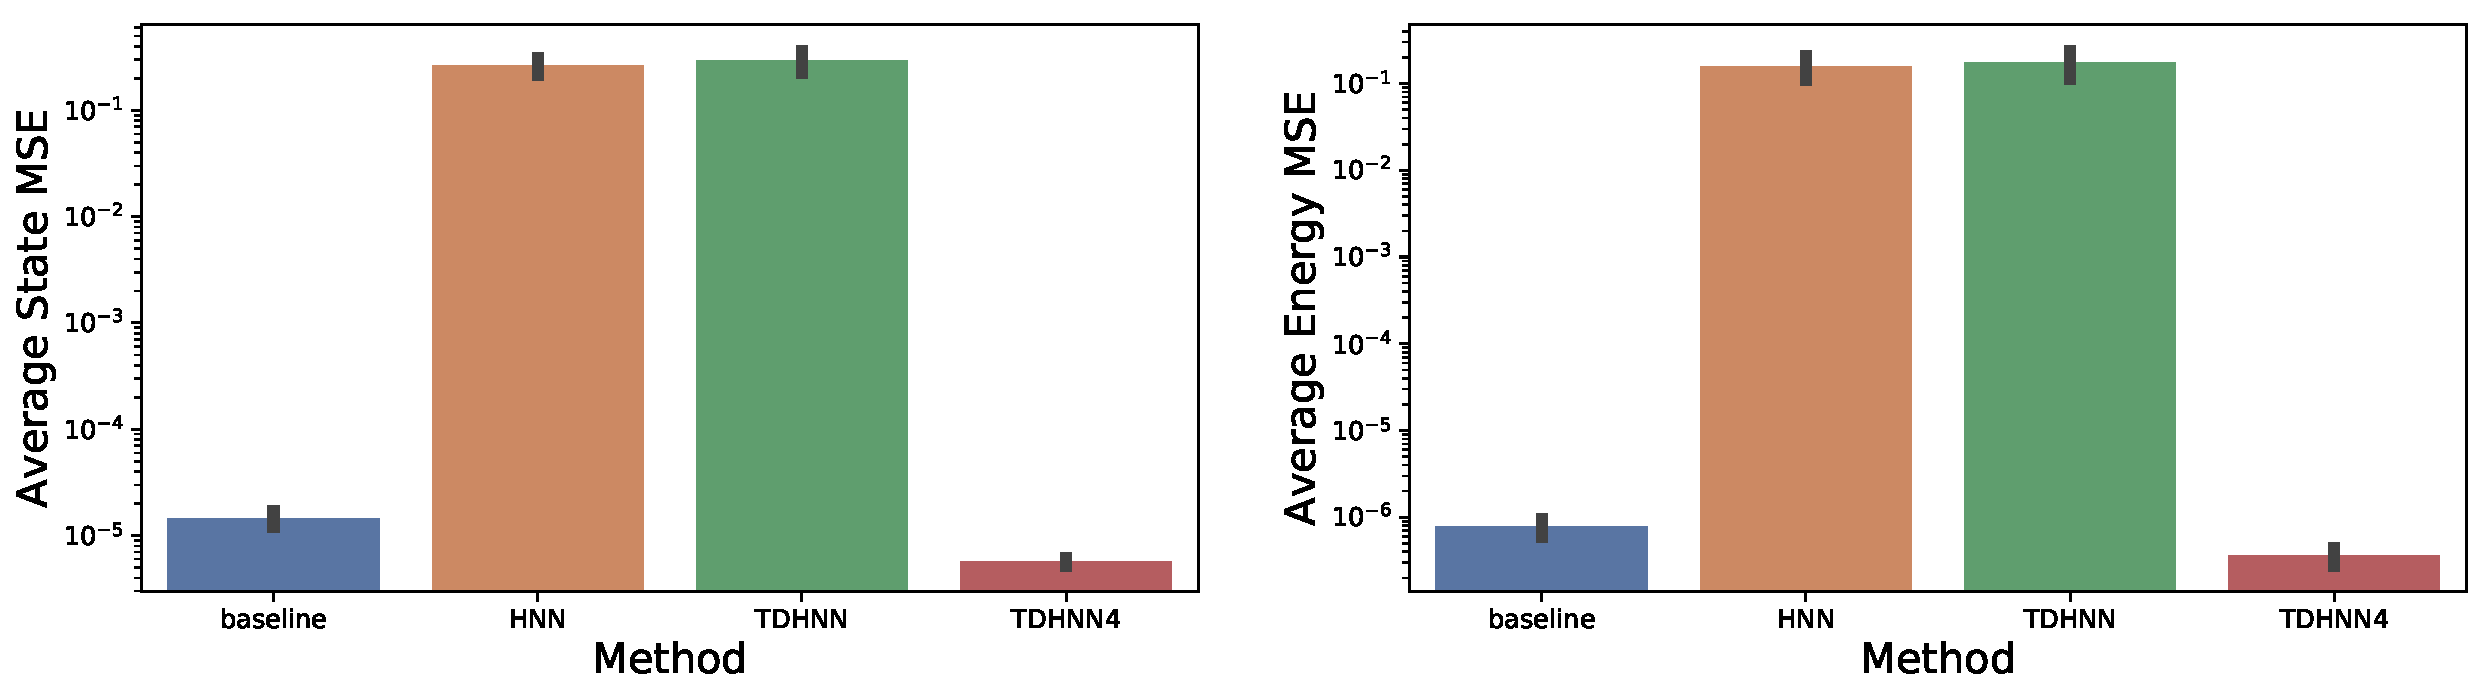
\includegraphics[width=0.49\textwidth]{figures/damped_1_errors.pdf}
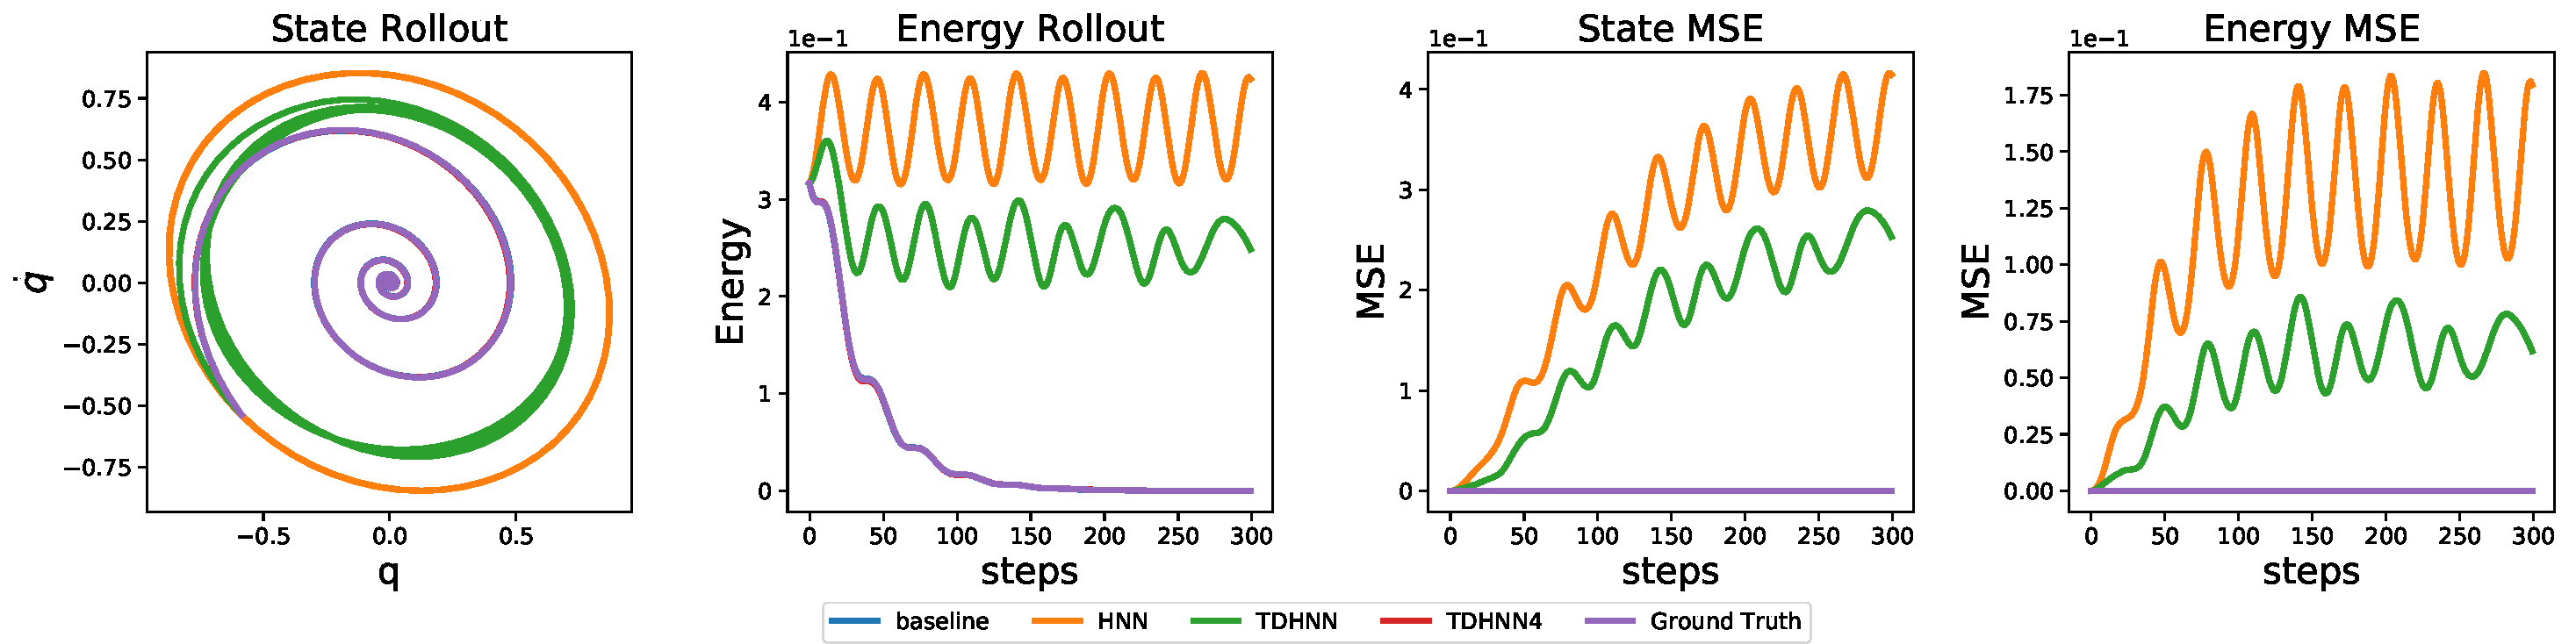
\includegraphics[width=0.49\textwidth]{figures/damped_1_pred.pdf}
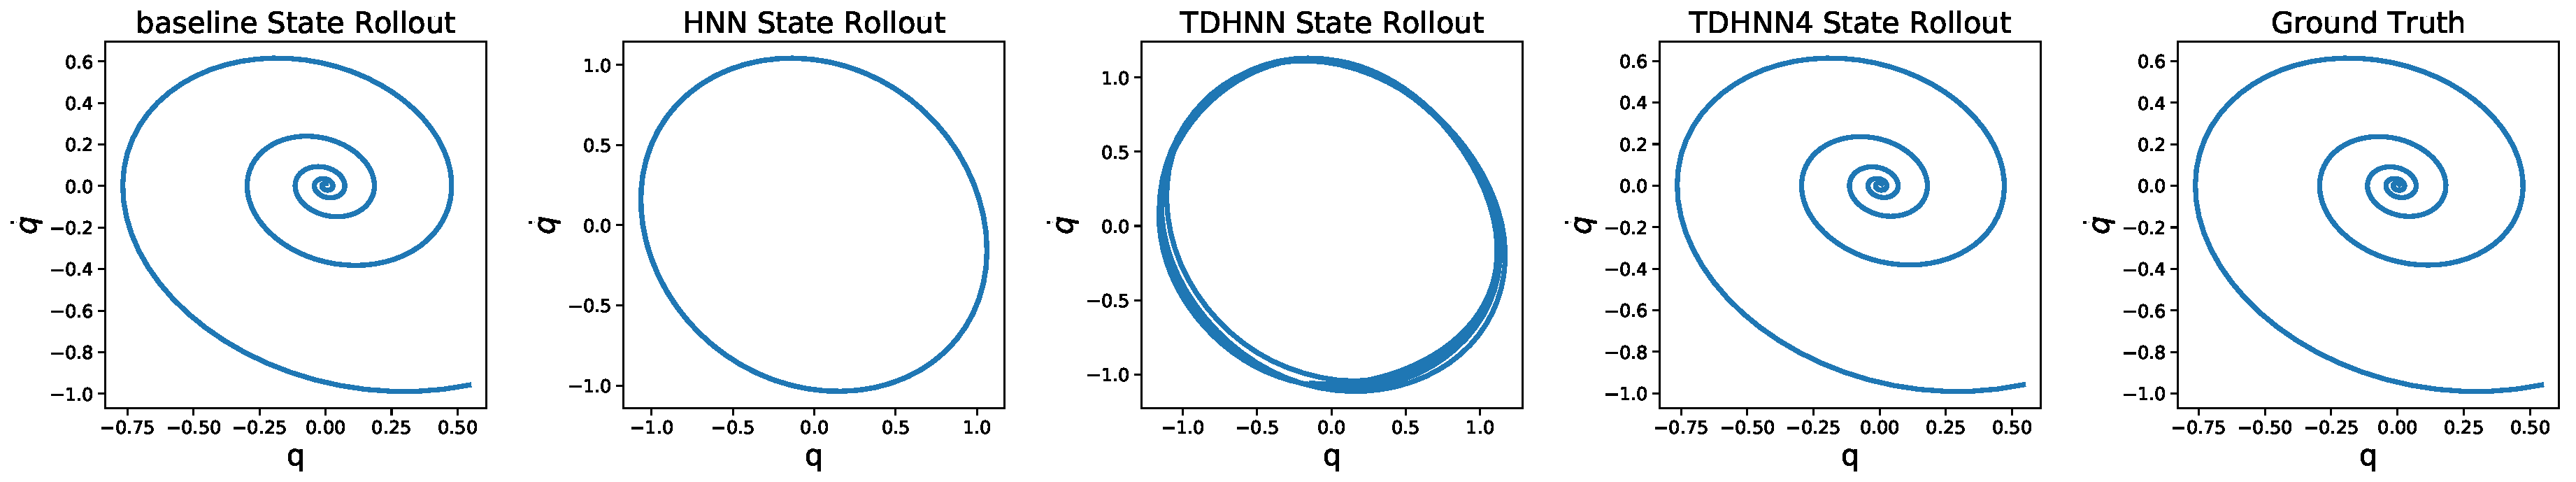
\includegraphics[width=0.49\textwidth]{figures/damped_rollout.pdf}
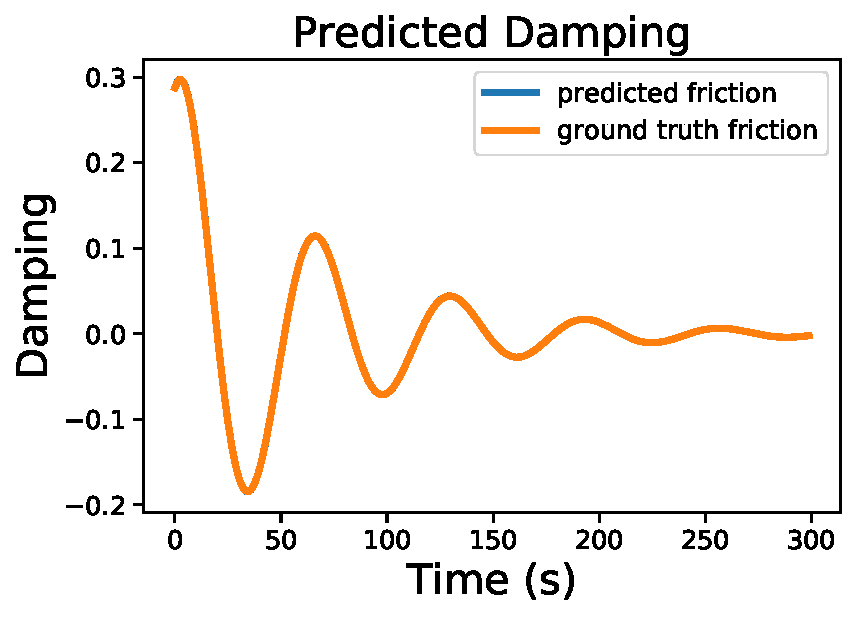
\includegraphics[width=0.49\textwidth]{figures/TDHNN4_damped_1.pdf}
\caption{Forced mass spring setting: HNN cannot learn the underlying dynamics as it has no explicit-time dependence. TDHNN4 shows the best performance as it explicitly learns a time-dependent force.}
\label{damped}
\end{figure}

We can see that both baseline NN and TDHNN4 recover the dynamics well, whereas HNN and TDHNN struggle to learn the damping as there is no direct way of learning a Hamiltonian with damping.

\subsection{Forced Mass Spring}

Typically, while we cannot write the Hamiltonian for a damped system, we can write one for a forced system. Here, we study 2 types of forced mass-spring systems. The first has the following Hamiltonian form:

\begin{equation}
\mathcal{H} = \frac{1}{2}k\mathbf{q}^2 + \frac{1}{2m}\mathbf{p}^2 - \mathbf{q}\mathbf{F_0}sin(\omega \mathbf{t}) 
\end{equation}

\begin{figure}[h!]
\centering
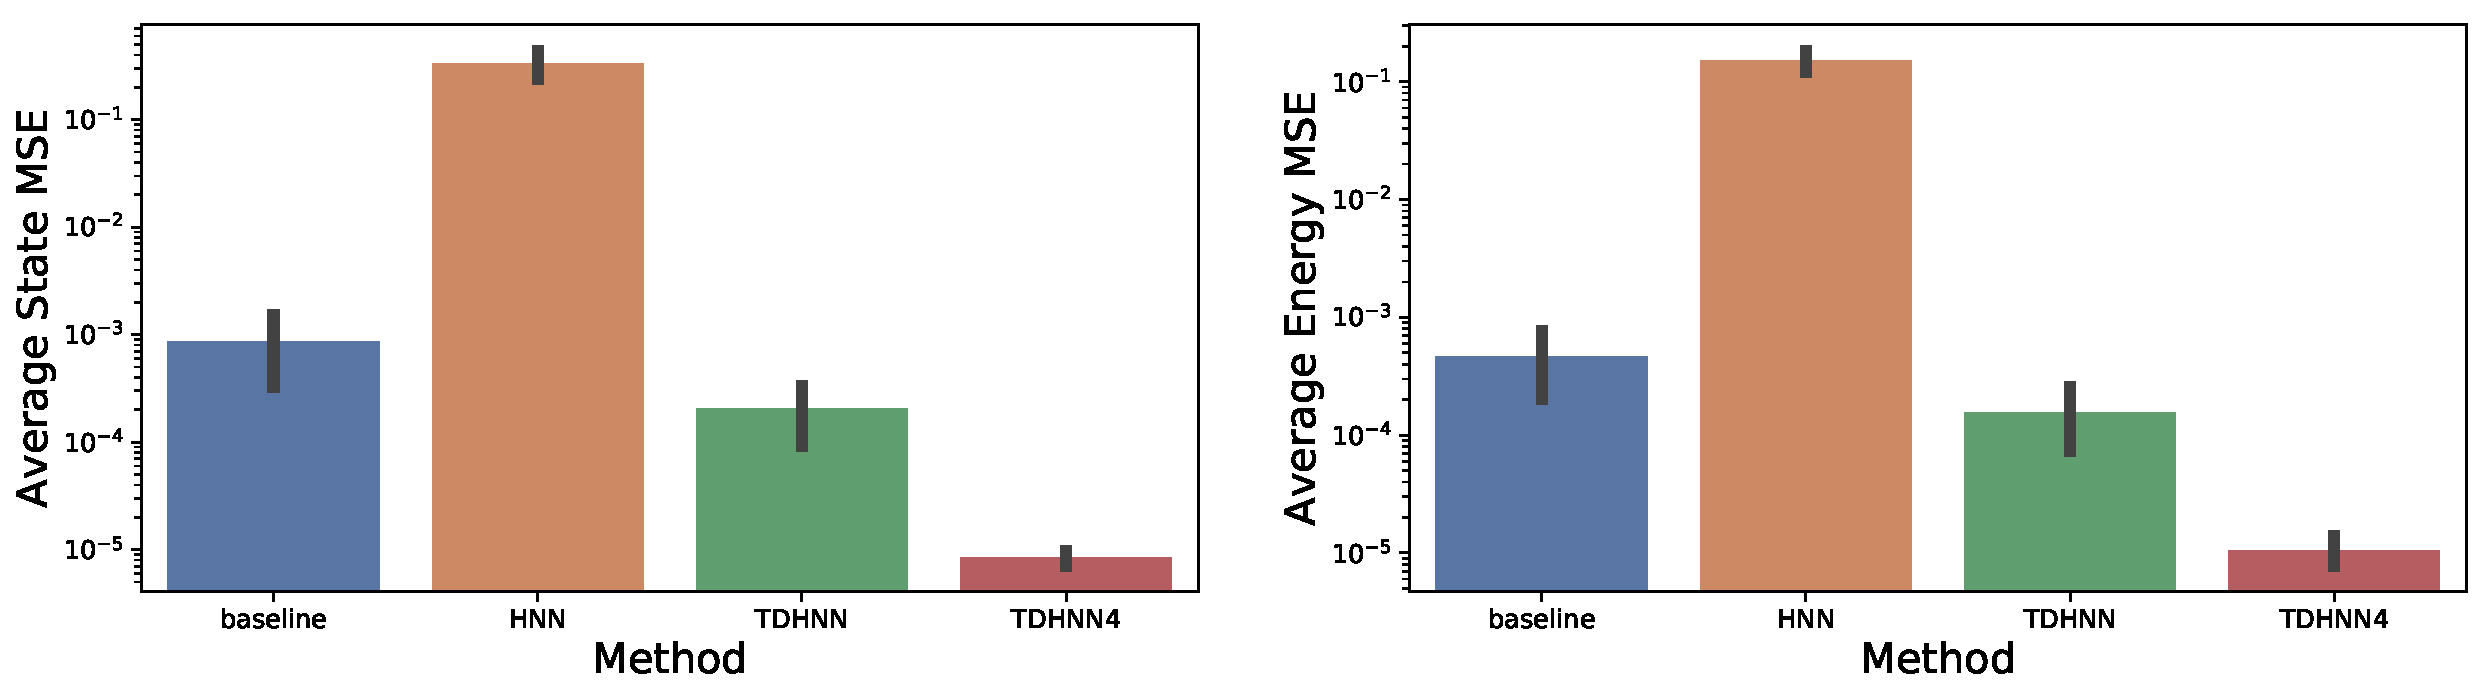
\includegraphics[width=0.49\textwidth]{figures/mass_spring_forced_1_errors.pdf}
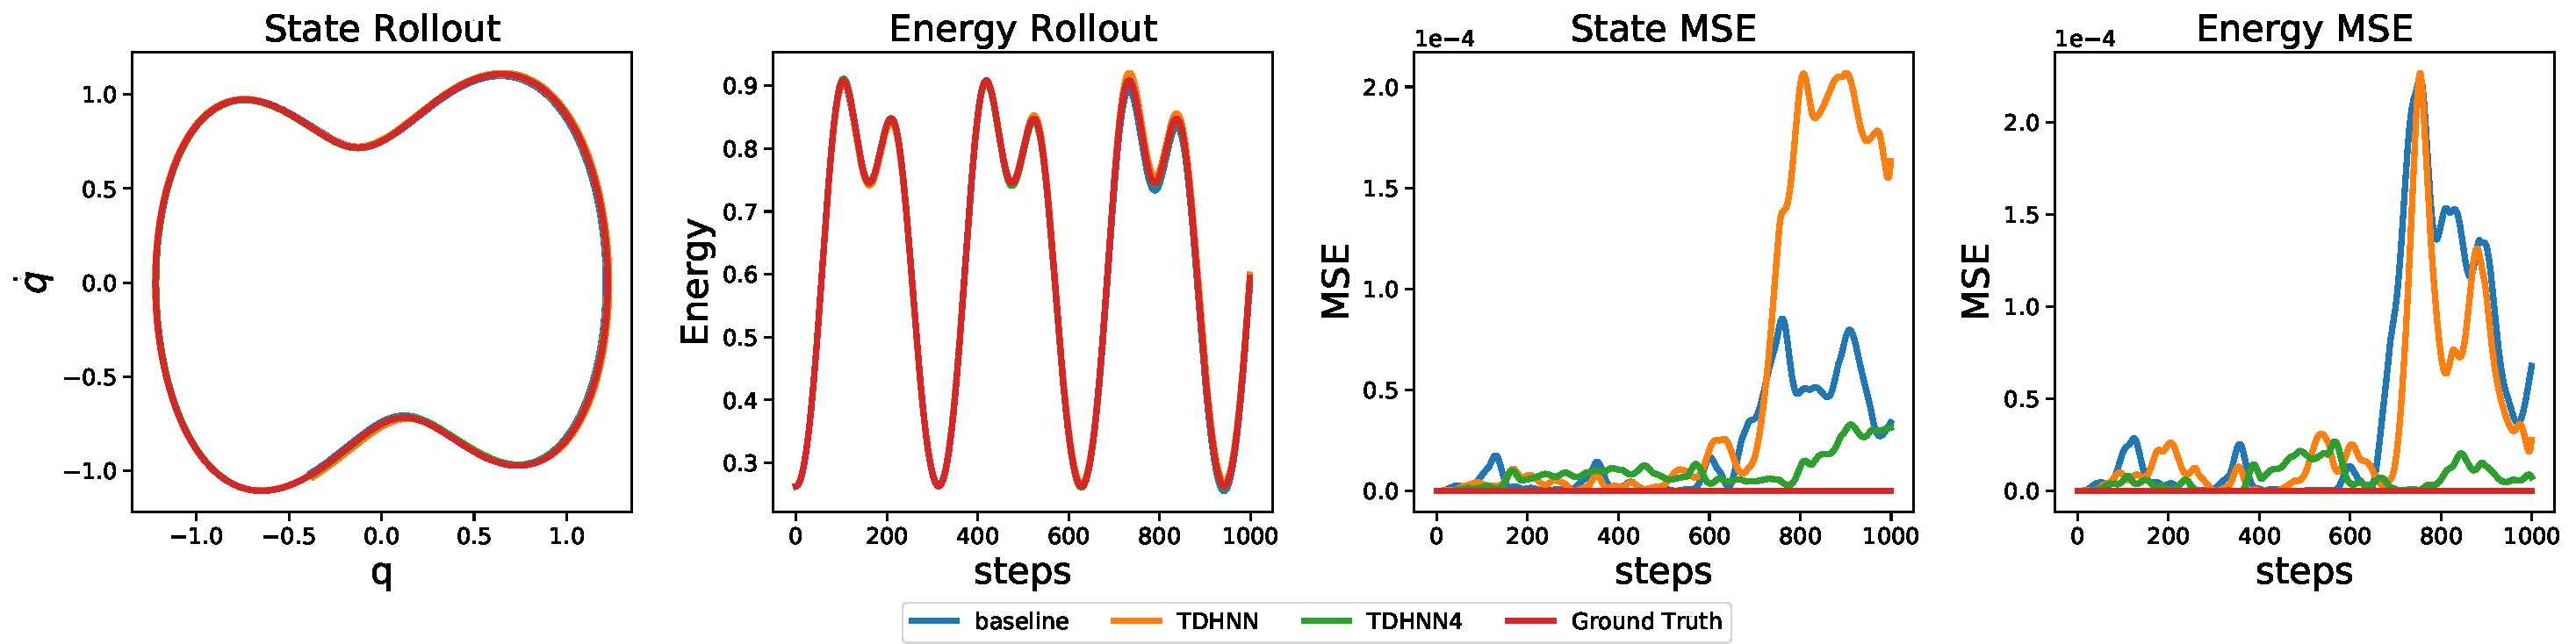
\includegraphics[width=0.49\textwidth]{figures/mass_spring_forced_1_pred.pdf}
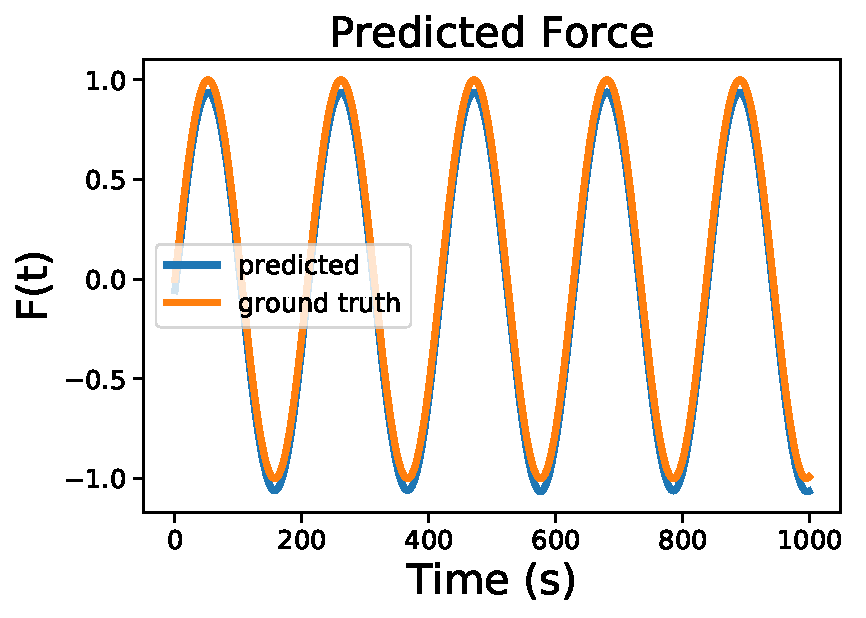
\includegraphics[width=0.49\textwidth]{figures/TDHNN4_mass_spring_force_1.pdf}
\caption{Forced mass spring setting: HNN cannot learn the underlying dynamics as it has no explicit-time dependence. TDHNN4 shows the best performance as it explicitly learns a time-dependent force.}
\end{figure}

The second has this Hamiltonian form:

\begin{equation}
\mathcal{H} = \frac{1}{2}k\mathbf{q}^2 + \frac{1}{2m}\mathbf{p}^2 - \mathbf{q}\mathbf{F_0}sin(\omega \mathbf{t})sin(2\omega \mathbf{t})
\end{equation}

\begin{figure}[h!]
\centering
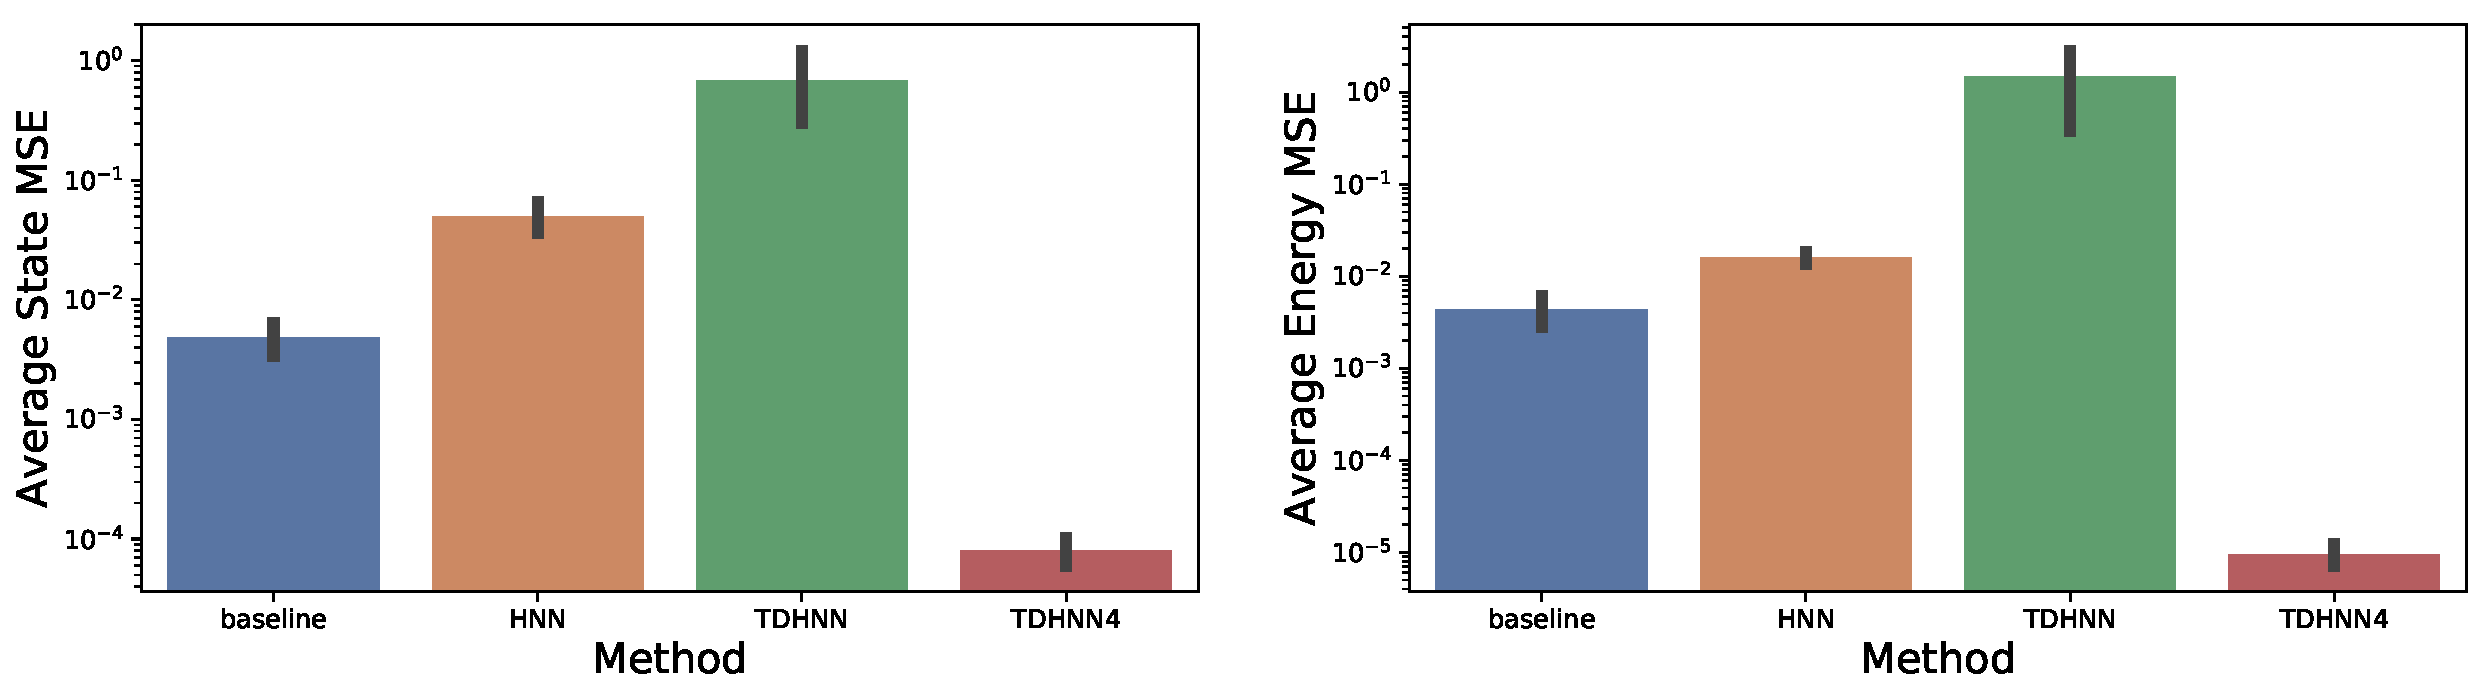
\includegraphics[width=0.49\textwidth]{figures/mass_spring_forced_2_errors.pdf}
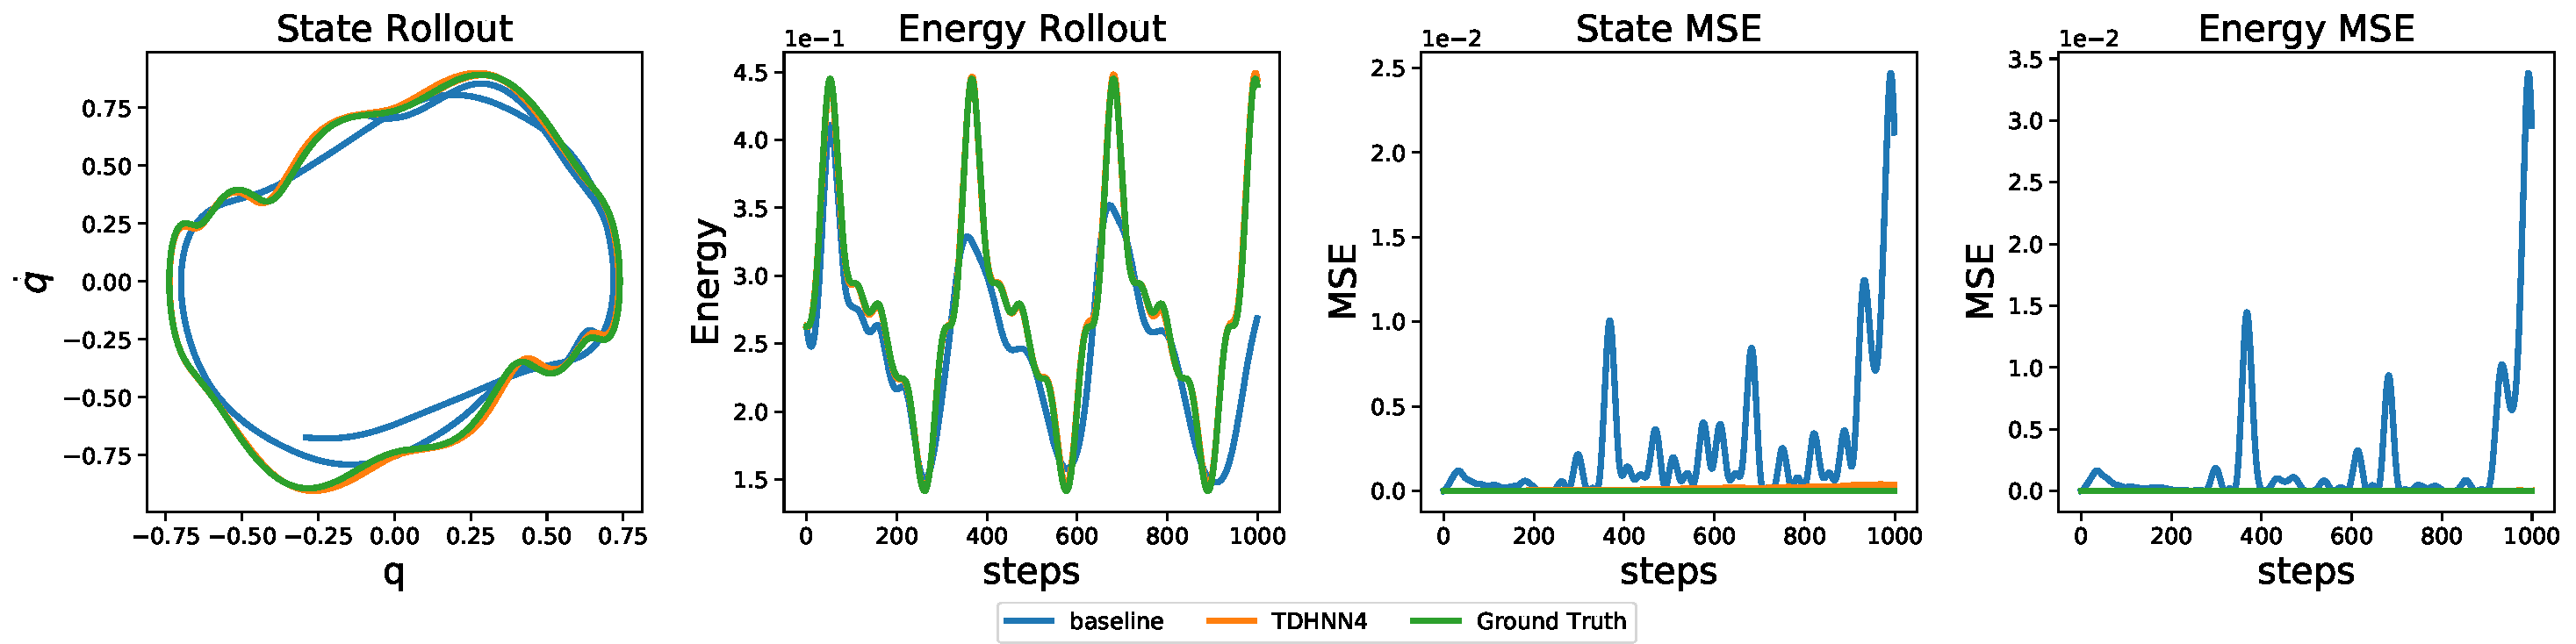
\includegraphics[width=0.49\textwidth]{figures/mass_spring_forced_2_pred.pdf}
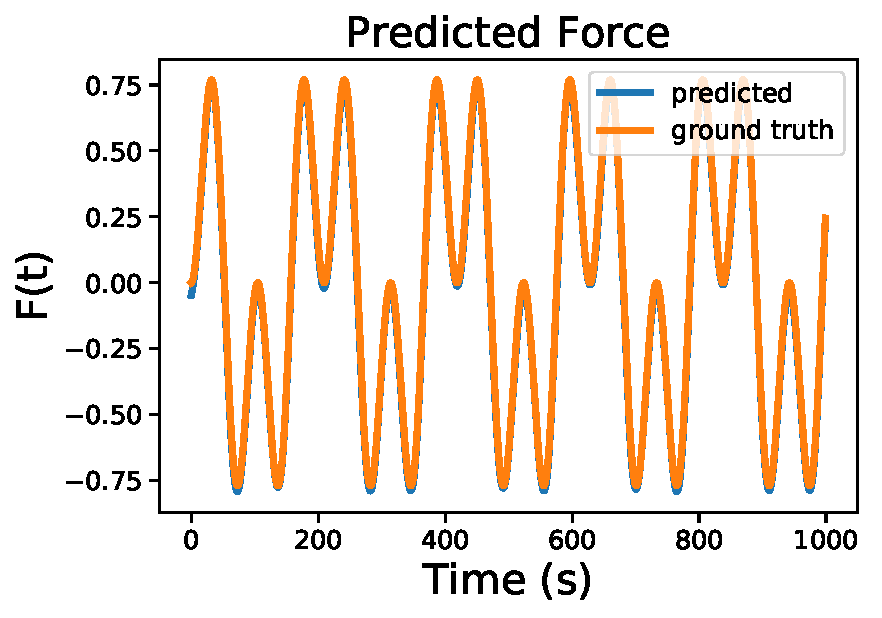
\includegraphics[width=0.49\textwidth]{figures/TDHNN4_mass_spring_force_2.pdf}
\caption{The time dependent force here is non-trivial, but TDHNN4 shows it can recover it precisely.}
\end{figure}

In both settings, we use 20 initial conditions, where the state is sampled from a radii between 0.5 and 1.5. The states are rolled out to $T_{max}=10.01$ at a $\delta t = 0.01$. At inference, we compute the rollout of 25 trajectories, and report the average state and energy rollout MSE in the figures.

\subsection{Duffing}

The general duffing equation combines both the force and damping terms. Typically the equation is written as:

\begin{equation}
\ddot{\mathbf{q}} = -\delta \dot{\mathbf{q}} -\alpha \mathbf{q} -\beta \mathbf{q}^3 +\gamma \sin(\omega \mathbf{t}) 
\end{equation}

One can see that the unforced and undamped regular Hamiltonian of the duffing system would be:

\begin{equation}
\mathcal{H}_{reg} = \frac{\mathbf{p}^2}{2m}+ \alpha \frac{\mathbf{q}^2}{2} + \beta \frac{\mathbf{q}^4}{4}
\end{equation}

This Hamiltonian therefore has a potential that would either be a single or a double well. A combination of parameters $\alpha,\beta,\delta,\gamma,\omega$ will make the duffing system either chaotic or non-chaotic. We study both regimes.

\subsubsection{Non-Chaotic}

Given a set of initial parameters where $\alpha =-1,\beta=1,\delta=0.3,\gamma=0.2,\omega=1.2$ we can obtain training data for the non-chaotic regime of the duffing equation. We uniformly sample initial conditions in $[-1,1]^2$. We use 25 initial conditions for training, rolled out to $T_{max}=10.01$ and $\delta t =0.01$ for the non-chaotice. 


\begin{figure}[h!]
\centering
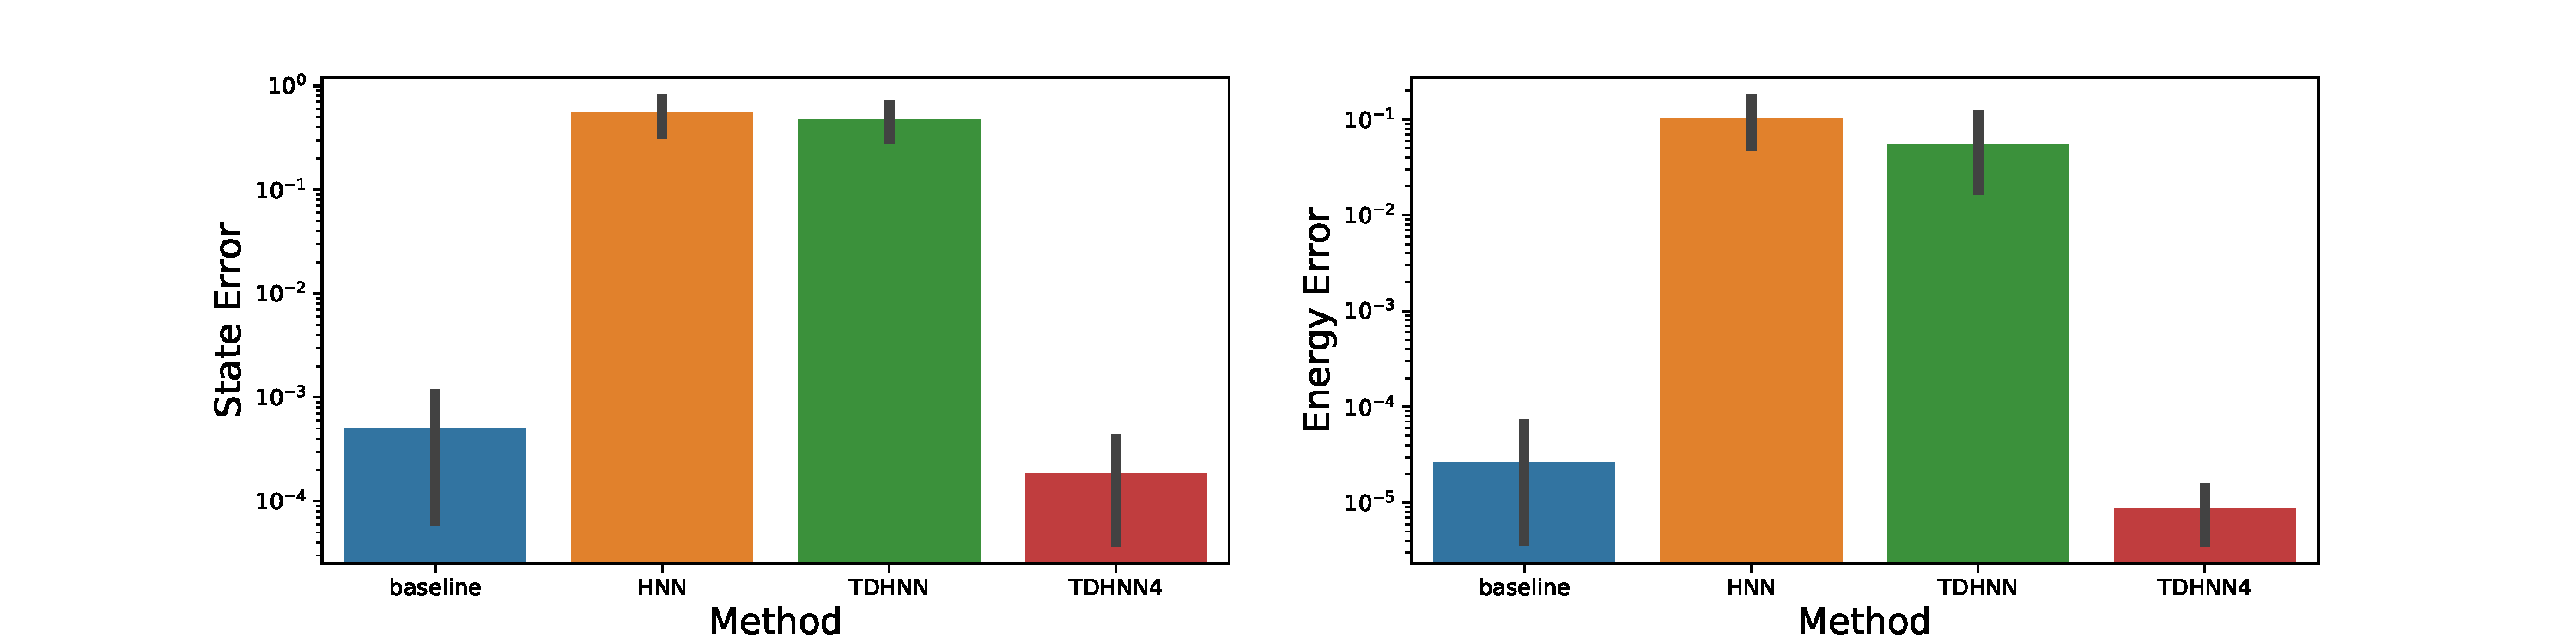
\includegraphics[width=0.5\textwidth]{figures/duffing_1_errors.pdf}
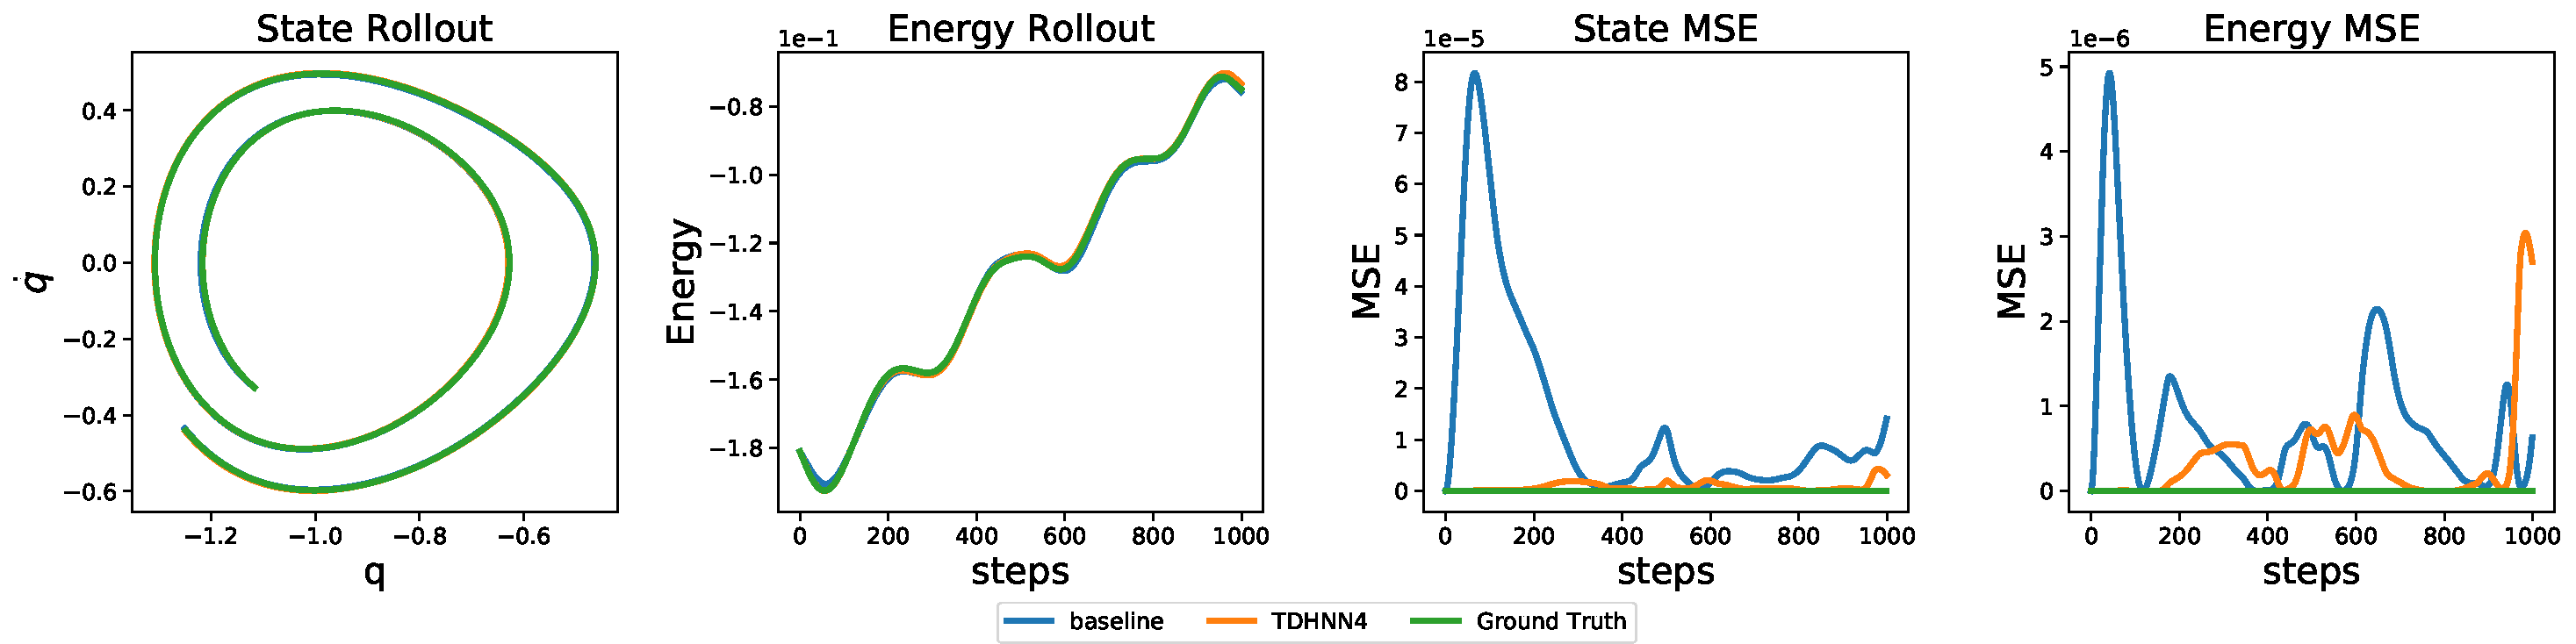
\includegraphics[width=0.49\textwidth]{figures/duffing_1_pred.pdf}
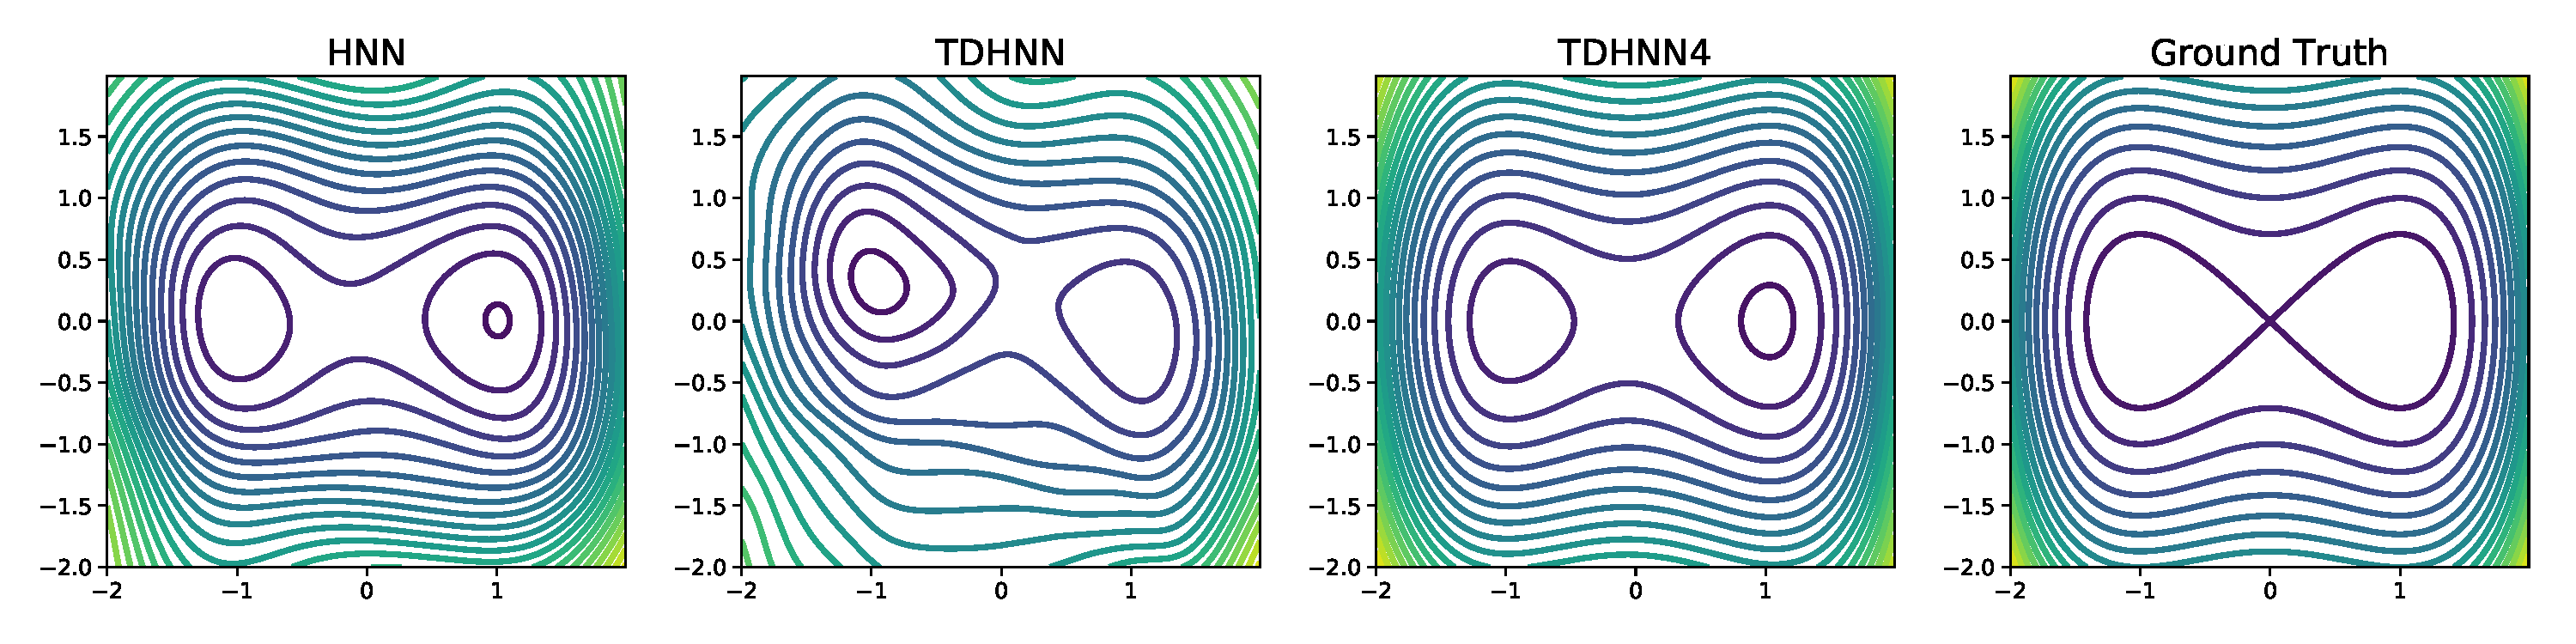
\includegraphics[width=0.49\textwidth]{figures/duffing_ham_1.pdf}
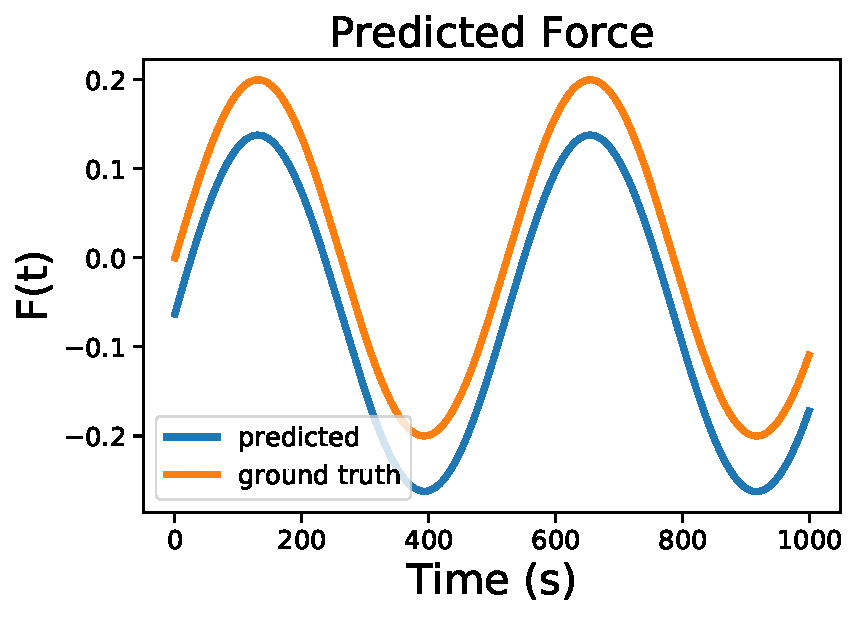
\includegraphics[width=0.49\textwidth]{figures/TDHNN4_duffing_1.pdf}
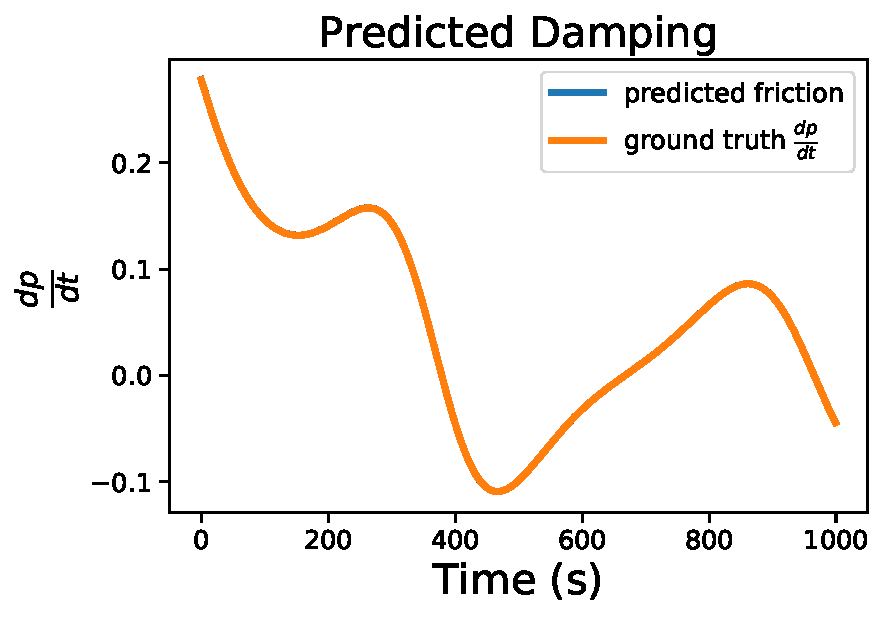
\includegraphics[width=0.4\textwidth]{figures/TDHNN4_duffing_damp_1.pdf}
\caption{baseline NN and TDHNN4 both perform really well in this setting. With TDHNN4 we are also able to extract the ground truth force and damping coefficient. The predicted Hamiltonian also visually appears closer to the ground truth in comparison to HNN or TDHNN.}
\end{figure}

\subsubsection{Chaotic}

In the chaotic regime we use the following parameters:
$\alpha =1,\beta=1,\delta=0.1,\gamma=0.39,\omega=1.4$. 

Training Data: 20 initial conditions, sampled uniformly in $[-1,1]^2$ each rolled out for one period $T=2\pi/\omega$ where $\delta t = T/100$. This results in 2000 training points.

Testing: we test the system on a single initial condition, rolled out to $T_{max} = 18,000$ with the same $\delta t$ as training. One additional change we make at inference is a modification to the time variable which is fed in. We work under the assumption that we have explicit knowledge of the period, and as such, we modulo the time variable with the period. This is necessary as the models are not explicitly trained on time steps beyond $T$. Using the unchanged time, our model predictions rapidly diverge from the ground truth. Our results are visually presented in Fig.\ref{fig.chaos}.  
\subsection{Relativity}

We investigate the duffing equation with a relativistic kinetic energy term. The general Hamiltonian form is:

\begin{equation}
\mathcal{H} =  c\sqrt{\mathbf{p}^2 +m^2c^2} + \frac{\alpha}{2}\mathbf{q}^2 +\frac{\beta}{4}\mathbf{q}^4 - \mathbf{q}\mathbf{F_0}sin(\omega \mathbf{t})
\end{equation}

where c, the speed of light is typically set to 1. For simplicity, we also set $m=1$ though our framework naturally accounts for other values.

\section{Discussion}

\section{Conclusion}



\begin{table*}[ht!]
\caption{Test Rollout MSE} 
\centering % centering table
\resizebox{\textwidth}{!}{\begin{tabular}{c  cc cc cc cc cc} % creating eight columns
\hline\hline %inserting double-line
\multirow{2}{*}{Method}&\multicolumn{2}{c}{Ideal Mass Spring}&\multicolumn{2}{c}{Damped Mass Spring} & \multicolumn{2}{c}{Forced Mass Spring (1)} &\multicolumn{2}{c}{Forced Mass Spring (2)} & \multicolumn{2}{c}{Duffing Non-Chaotic} \\
\cline{2-11} % inserts single-line
 & State & Energy & State & Energy & State & Energy & State & Energy & State & Energy \\
\hline
Baseline NN &\\ % Entering row contents
HNN &\\
TDHNN &\\
TDHNN4 &
\\% [1ex] adds vertical space
\hline % inserts single-line
\end{tabular}}
\label{tab:tests}
\end{table*}

\pagebreak

\bibliography{references.bib}
\end{document}
